\documentclass{article}
\usepackage[utf8]{inputenc}

\title{Constructive Temporal Logic, Categorically}
\author{Valeria de Paiva \and Harley Eades III}
\date{July 2016}

\usepackage{natbib}
\usepackage{graphicx}
\usepackage{amssymb, amsthm, amsmath, stmaryrd}
\usepackage{mathpartir}
\usepackage{mdframed}           % For the boxes around the systems.
\usepackage{cmll}
\usepackage[barr]{xy}

%% This renames Barr's \Diamond command so that it doesn't conflict
%% with our modality symbols.
\let\BDiamond\Diamond
\let\Diamond\relax
\newcommand{\bLozenge}{\mathbin{\blacklozenge}}
%% This renames Barr's \to to \mto.  This allows us to use \to for imp
%% and \mto for a inline morphism.
\let\mto\to
\let\to\relax
\newcommand{\to}{\rightarrow}

\usepackage{wasysym}
\usepackage{proof}
\usepackage{enumerate}
\usepackage{todonotes}
\usepackage{hyperref}
\usepackage{graphicx}

\let\b\relax
\let\d\relax
\let\t\relax

\renewcommand{\Box}{\oblong}
\newcommand{\BBox}{\blacksquare}
\newcommand{\BDia}{\mathbin{\blacklozenge}}
\def\sem#1{[\hspace{-0.05cm}[#1]\hspace{-0.05cm}]}

\newcommand{\F}{\mathop{\textbf{F}}}
\renewcommand{\P}{\mathop{\textbf{P}}}
\newcommand{\G}{\mathop{\textbf{G}}}
\renewcommand{\H}{\mathop{\textbf{H}}}

\newcommand{\cat}[1]{\mathcal{#1}}
\newcommand{\pd}[0]{\times}
\newcommand{\ihom}[0]{\rightarrow}
\newcommand{\st}[2]{\mathsf{st}_{#1,#2}}
\newcommand{\id}[0]{\mathsf{id}}
\newcommand{\b}[1]{\mathsf{b}_{#1}}
\newcommand{\d}[1]{\mathsf{d}_{#1}}
\newcommand{\m}[1]{\mathsf{m}_{#1}}
\newcommand{\n}[1]{\mathsf{n}_{#1}}
\newcommand{\p}[1]{\mathsf{p}_{#1}}
\newcommand{\q}[1]{\mathsf{q}_{#1}}
\newcommand{\t}[0]{\mathsf{t}}
\newcommand{\limp}[0]{\multimap}
\newcommand{\Hom}[3]{\mathsf{Hom}_{#1}(#2,#3)}

\def\cW{\color{white}}

%% Begin Ott
% generated by Ott 0.25 from: ott/TCS4.ott
\newcommand{\TLLdrule}[4][]{{\displaystyle\frac{\begin{array}{l}#2\end{array}}{#3}\quad\TLLdrulename{#4}}}
\newcommand{\TLLusedrule}[1]{\[#1\]}
\newcommand{\TLLpremise}[1]{ #1 \\}
\newenvironment{TLLdefnblock}[3][]{ \framebox{\mbox{#2}} \quad #3 \\[0pt]}{}
\newenvironment{TLLfundefnblock}[3][]{ \framebox{\mbox{#2}} \quad #3 \\[0pt]\begin{displaymath}\begin{array}{l}}{\end{array}\end{displaymath}}
\newcommand{\TLLfunclause}[2]{ #1 \equiv #2 \\}
\newcommand{\TLLnt}[1]{\mathit{#1}}
\newcommand{\TLLmv}[1]{\mathit{#1}}
\newcommand{\TLLkw}[1]{\mathbf{#1}}
\newcommand{\TLLsym}[1]{#1}
\newcommand{\TLLcom}[1]{\text{#1}}
\newcommand{\TLLdrulename}[1]{\textsc{#1}}
\newcommand{\TLLcomplu}[5]{\overline{#1}^{\,#2\in #3 #4 #5}}
\newcommand{\TLLcompu}[3]{\overline{#1}^{\,#2<#3}}
\newcommand{\TLLcomp}[2]{\overline{#1}^{\,#2}}
\newcommand{\TLLgrammartabular}[1]{\begin{supertabular}{llcllllll}#1\end{supertabular}}
\newcommand{\TLLmetavartabular}[1]{\begin{supertabular}{ll}#1\end{supertabular}}
\newcommand{\TLLrulehead}[3]{$#1$ & & $#2$ & & & \multicolumn{2}{l}{#3}}
\newcommand{\TLLprodline}[6]{& & $#1$ & $#2$ & $#3 #4$ & $#5$ & $#6$}
\newcommand{\TLLfirstprodline}[6]{\TLLprodline{#1}{#2}{#3}{#4}{#5}{#6}}
\newcommand{\TLLlongprodline}[2]{& & $#1$ & \multicolumn{4}{l}{$#2$}}
\newcommand{\TLLfirstlongprodline}[2]{\TLLlongprodline{#1}{#2}}
\newcommand{\TLLbindspecprodline}[6]{\TLLprodline{#1}{#2}{#3}{#4}{#5}{#6}}
\newcommand{\TLLprodnewline}{\\}
\newcommand{\TLLinterrule}{\\[5.0mm]}
\newcommand{\TLLafterlastrule}{\\}
\newcommand{\TLLmetavars}{
\TLLmetavartabular{
 $ \mathit{termvar} ,\, \mathit{x} ,\, \mathit{y} $ & \TLLcom{term variable} \\
 $ \TLLmv{index} ,\, \TLLmv{i} ,\, \TLLmv{j} ,\, \TLLmv{k} $ &  \\
}}

\newcommand{\TLLterm}{
\TLLrulehead{\TLLnt{term}  ,\ \TLLnt{t}  ,\ \TLLnt{r}  ,\ \TLLnt{s}  ,\ \TLLnt{n}}{::=}{\TLLcom{term}}\TLLprodnewline
\TLLfirstprodline{|}{\mathit{x}}{}{}{}{\TLLcom{variable}}\TLLprodnewline
\TLLprodline{|}{ \mathsf{contra} }{}{}{}{}\TLLprodnewline
\TLLprodline{|}{ \lambda  \mathit{x}  :  \TLLnt{T} . \TLLnt{t} }{}{}{}{\TLLcom{unary functions}}\TLLprodnewline
\TLLprodline{|}{\TLLnt{t_{{\mathrm{1}}}} \, \TLLnt{t_{{\mathrm{2}}}}}{}{}{}{\TLLcom{function application}}\TLLprodnewline
\TLLprodline{|}{\mathsf{unbox}_\Box\, \, \TLLnt{t}}{}{}{}{}\TLLprodnewline
\TLLprodline{|}{\mathsf{unbox}_\blacksquare\, \, \TLLnt{t}}{}{}{}{}\TLLprodnewline
\TLLprodline{|}{\Box \, \TLLnt{t}}{}{}{}{\TLLcom{past necessity functor}}\TLLprodnewline
\TLLprodline{|}{\Diamond \, \TLLnt{t}}{}{}{}{\TLLcom{past possibility functor}}\TLLprodnewline
\TLLprodline{|}{\blacksquare \, \TLLnt{t}}{}{}{}{\TLLcom{necessity functor}}\TLLprodnewline
\TLLprodline{|}{\mathbin{\blacklozenge} \, \TLLnt{t}}{}{}{}{\TLLcom{possibility functor}}\TLLprodnewline
\TLLprodline{|}{ \mathsf{adj_R}\,\blacklozenge  \mathit{y}  =  \mathit{x} \,\mathsf{in}\,\Box  \TLLnt{t} }{}{}{}{}\TLLprodnewline
\TLLprodline{|}{ \mathsf{adj_L}\,\blacklozenge  \mathit{y}  =  \mathit{x} \,\mathsf{in}\, \TLLnt{t} }{}{}{}{}\TLLprodnewline
\TLLprodline{|}{ \mathsf{let}_\Box\, \Gamma \,\mathsf{be}\, \TLLnt{t_{{\mathrm{1}}}} \,\mathsf{in}\, \TLLnt{t_{{\mathrm{2}}}} }{}{}{}{\TLLcom{past necessity elim}}\TLLprodnewline
\TLLprodline{|}{ \mathsf{let}_\blacksquare\, \Gamma \,\mathsf{be}\, \TLLnt{t_{{\mathrm{1}}}} \,\mathsf{in}\, \TLLnt{t_{{\mathrm{2}}}} }{}{}{}{\TLLcom{past necessity elim}}\TLLprodnewline
\TLLprodline{|}{ \mathsf{let}\,\Diamond  \mathit{x} : \TLLnt{A} = \TLLnt{s}  \mid  \Gamma \,\mathsf{be}\, \TLLnt{t_{{\mathrm{1}}}} \,\mathsf{in}\, \TLLnt{t_{{\mathrm{2}}}} }{}{}{}{}\TLLprodnewline
\TLLprodline{|}{ \mathsf{let}\,\blacklozenge  \mathit{x} : \TLLnt{A} = \TLLnt{s}  \mid  \Gamma \,\mathsf{be}\, \TLLnt{t_{{\mathrm{1}}}} \,\mathsf{in}\, \TLLnt{t_{{\mathrm{2}}}} }{}{}{}{}\TLLprodnewline
\TLLprodline{|}{\TLLsym{[}  \TLLnt{t_{{\mathrm{1}}}}  \TLLsym{/}  \TLLnt{t}  \TLLsym{]}  \TLLnt{t_{{\mathrm{2}}}}} {\textsf{M}}{}{}{}\TLLprodnewline
\TLLprodline{|}{\TLLsym{(}  \TLLnt{t}  \TLLsym{)}} {\textsf{S}}{}{}{}\TLLprodnewline
\TLLprodline{|}{ \TLLnt{t} } {\textsf{M}}{}{}{}\TLLprodnewline
\TLLprodline{|}{\TLLnt{r} \, \TLLkw{R}} {\textsf{M}}{}{}{}\TLLprodnewline
\TLLprodline{|}{ \mathsf{let}\,\mathbin{M}  \TLLnt{t_{{\mathrm{1}}}} : \TLLnt{T}  =  \TLLnt{t_{{\mathrm{2}}}} \,\mathsf{in}\, \TLLnt{t_{{\mathrm{3}}}} } {\textsf{M}}{}{}{}\TLLprodnewline
\TLLprodline{|}{ \overrightarrow{ \TLLnt{t} } } {\textsf{M}}{}{}{}\TLLprodnewline
\TLLprodline{|}{ \mathbin{M}  \TLLnt{t} } {\textsf{M}}{}{}{}\TLLprodnewline
\TLLprodline{|}{\TLLnt{t_{{\mathrm{1}}}}  \TLLsym{,} \, ... \, \TLLsym{,}  \TLLnt{t_{\TLLmv{k}}}} {\textsf{M}}{}{}{}\TLLprodnewline
\TLLprodline{|}{\TLLsym{[}  \TLLnt{t_{{\mathrm{1}}}}  \TLLsym{/}  \mathit{x_{{\mathrm{1}}}}  \TLLsym{]} \, ... \, \TLLsym{[}  \TLLnt{t_{\TLLmv{k}}}  \TLLsym{/}  \mathit{x_{\TLLmv{k}}}  \TLLsym{]}  \TLLnt{t}} {\textsf{M}}{}{}{}}

\newcommand{\TLLform}{
\TLLrulehead{\TLLnt{form}  ,\ \TLLnt{type}  ,\ \TLLnt{A}  ,\ \TLLnt{B}  ,\ \TLLnt{C}  ,\ \TLLnt{T}}{::=}{\TLLcom{formula and type}}\TLLprodnewline
\TLLfirstprodline{|}{\perp}{}{}{}{\TLLcom{false or the empty type}}\TLLprodnewline
\TLLprodline{|}{\Box \, \TLLnt{A}}{}{}{}{\TLLcom{past necessity}}\TLLprodnewline
\TLLprodline{|}{\blacksquare \, \TLLnt{A}}{}{}{}{\TLLcom{necessity}}\TLLprodnewline
\TLLprodline{|}{\Diamond \, \TLLnt{A}}{}{}{}{\TLLcom{past possibility}}\TLLprodnewline
\TLLprodline{|}{\mathbin{\blacklozenge} \, \TLLnt{A}}{}{}{}{\TLLcom{possibility}}\TLLprodnewline
\TLLprodline{|}{ \TLLnt{A}  \times  \TLLnt{B} }{}{}{}{}\TLLprodnewline
\TLLprodline{|}{\TLLnt{A}  \to  \TLLnt{B}}{}{}{}{\TLLcom{implication}}\TLLprodnewline
\TLLprodline{|}{ \TLLnt{A}  \limp  \TLLnt{B} }{}{}{}{}\TLLprodnewline
\TLLprodline{|}{\mathsf{F} \, \TLLnt{X}}{}{}{}{}\TLLprodnewline
\TLLprodline{|}{ \mathbin{M}  \TLLnt{A} } {\textsf{M}}{}{}{}}

\newcommand{\TLLiform}{
\TLLrulehead{\TLLnt{iform}  ,\ \TLLnt{X}  ,\ \TLLnt{Y}  ,\ \TLLnt{Z}}{::=}{}\TLLprodnewline
\TLLfirstprodline{|}{\TLLnt{X}  \to  \TLLnt{Y}}{}{}{}{}\TLLprodnewline
\TLLprodline{|}{\mathsf{G} \, \TLLnt{A}}{}{}{}{}}

\newcommand{\TLLG}{
\TLLrulehead{\Gamma  ,\ \Delta}{::=}{\TLLcom{type context}}\TLLprodnewline
\TLLfirstprodline{|}{\emptyset}{}{}{}{\TLLcom{empty context}}\TLLprodnewline
\TLLprodline{|}{\TLLnt{A}}{}{}{}{\TLLcom{formula el}}\TLLprodnewline
\TLLprodline{|}{\mathit{x}  \TLLsym{:}  \TLLnt{T}}{}{}{}{\TLLcom{typed el}}\TLLprodnewline
\TLLprodline{|}{\Gamma  \TLLsym{,}  \Gamma'}{}{}{}{\TLLcom{append}}\TLLprodnewline
\TLLprodline{|}{\Gamma_{{\mathrm{1}}}  \TLLsym{,} \, ... \, \TLLsym{,}  \Gamma_{\TLLmv{k}}} {\textsf{M}}{}{}{}}

\newcommand{\TLLTh}{
\TLLrulehead{\Theta  ,\ \Phi}{::=}{}\TLLprodnewline
\TLLfirstprodline{|}{\emptyset}{}{}{}{}\TLLprodnewline
\TLLprodline{|}{\TLLnt{X}}{}{}{}{}\TLLprodnewline
\TLLprodline{|}{\Theta_{{\mathrm{1}}}  \TLLsym{,}  \Theta_{{\mathrm{2}}}}{}{}{}{}}

\newcommand{\TLLterminals}{
\TLLrulehead{\TLLnt{terminals}}{::=}{}\TLLprodnewline
\TLLfirstprodline{|}{ \mathsf{F} }{}{}{}{}\TLLprodnewline
\TLLprodline{|}{ \mathsf{G} }{}{}{}{}\TLLprodnewline
\TLLprodline{|}{ \mathsf{unbox}_\Box\, }{}{}{}{}\TLLprodnewline
\TLLprodline{|}{ \mathsf{unbox}_\blacksquare\, }{}{}{}{}\TLLprodnewline
\TLLprodline{|}{ \emptyset }{}{}{}{}\TLLprodnewline
\TLLprodline{|}{ \perp }{}{}{}{}\TLLprodnewline
\TLLprodline{|}{ \vdash }{}{}{}{}\TLLprodnewline
\TLLprodline{|}{ \Box }{}{}{}{}\TLLprodnewline
\TLLprodline{|}{ \blacksquare }{}{}{}{}\TLLprodnewline
\TLLprodline{|}{ \Diamond }{}{}{}{}\TLLprodnewline
\TLLprodline{|}{ \mathbin{\blacklozenge} }{}{}{}{}\TLLprodnewline
\TLLprodline{|}{ \to }{}{}{}{}\TLLprodnewline
\TLLprodline{|}{ \quad } {\textsf{M}}{}{}{}\TLLprodnewline
\TLLprodline{|}{ \vdash_{\mathcal{C} } }{}{}{}{}\TLLprodnewline
\TLLprodline{|}{ \vdash_{\mathcal{L} } }{}{}{}{}}

\newcommand{\TLLformula}{
\TLLrulehead{\TLLnt{formula}}{::=}{}\TLLprodnewline
\TLLfirstprodline{|}{\TLLnt{judgement}}{}{}{}{}\TLLprodnewline
\TLLprodline{|}{\TLLnt{formula_{{\mathrm{1}}}}  \quad  \TLLnt{formula_{{\mathrm{2}}}}} {\textsf{M}}{}{}{}\TLLprodnewline
\TLLprodline{|}{ \TLLnt{formula} } {\textsf{S}}{}{}{}\TLLprodnewline
\TLLprodline{|}{ M \in \{\Diamond, \mathbin{\blacklozenge} \} } {\textsf{M}}{}{}{}\TLLprodnewline
\TLLprodline{|}{\TLLnt{formula_{{\mathrm{1}}}}  \TLLsym{,} \, ... \, \TLLsym{,}  \TLLnt{formula_{\TLLmv{k}}}}{}{}{}{}}

\newcommand{\TLLJtype}{
\TLLrulehead{\TLLnt{Jtype}}{::=}{}\TLLprodnewline
\TLLfirstprodline{|}{\Theta  \vdash_{\mathcal{C} }  \TLLnt{Z}}{}{}{}{}\TLLprodnewline
\TLLprodline{|}{\Theta  \TLLsym{;}  \Gamma  \vdash_{\mathcal{L} }  \TLLnt{A}}{}{}{}{}\TLLprodnewline
\TLLprodline{|}{\Gamma  \vdash  \TLLnt{t}  \TLLsym{:}  \TLLnt{A}}{}{}{}{}\TLLprodnewline
\TLLprodline{|}{ \Gamma  \vdash  \TLLnt{t_{{\mathrm{1}}}}  =  \TLLnt{t_{{\mathrm{2}}}}  :  \TLLnt{A} }{}{}{}{}}

\newcommand{\TLLjudgement}{
\TLLrulehead{\TLLnt{judgement}}{::=}{}\TLLprodnewline
\TLLfirstprodline{|}{\TLLnt{Jtype}}{}{}{}{}}

\newcommand{\TLLuserXXsyntax}{
\TLLrulehead{\TLLnt{user\_syntax}}{::=}{}\TLLprodnewline
\TLLfirstprodline{|}{\mathit{termvar}}{}{}{}{}\TLLprodnewline
\TLLprodline{|}{\TLLmv{index}}{}{}{}{}\TLLprodnewline
\TLLprodline{|}{\TLLnt{term}}{}{}{}{}\TLLprodnewline
\TLLprodline{|}{\TLLnt{form}}{}{}{}{}\TLLprodnewline
\TLLprodline{|}{\TLLnt{iform}}{}{}{}{}\TLLprodnewline
\TLLprodline{|}{\Gamma}{}{}{}{}\TLLprodnewline
\TLLprodline{|}{\Theta}{}{}{}{}\TLLprodnewline
\TLLprodline{|}{\TLLnt{terminals}}{}{}{}{}\TLLprodnewline
\TLLprodline{|}{\TLLnt{formula}}{}{}{}{}}

\newcommand{\TLLgrammar}{\TLLgrammartabular{
\TLLterm\TLLinterrule
\TLLform\TLLinterrule
\TLLiform\TLLinterrule
\TLLG\TLLinterrule
\TLLTh\TLLinterrule
\TLLterminals\TLLinterrule
\TLLformula\TLLinterrule
\TLLJtype\TLLinterrule
\TLLjudgement\TLLinterrule
\TLLuserXXsyntax\TLLafterlastrule
}}

% defnss
% defns Jtype
%% defn iseq
\newcommand{\TLLdruleiXXCArleftName}[0]{\TLLdrulename{i\_CArleft}}
\newcommand{\TLLdruleiXXCArleft}[1]{\TLLdrule[#1]{%
\TLLpremise{\Theta  \vdash_{\mathcal{C} }  \TLLnt{X}  \quad  \TLLnt{Y}  \TLLsym{,}  \Phi  \vdash_{\mathcal{C} }  \TLLnt{Z}}%
}{
\Theta  \TLLsym{,}  \TLLnt{X}  \to  \TLLnt{Y}  \TLLsym{,}  \Phi  \vdash_{\mathcal{C} }  \TLLnt{Z}}{%
{\TLLdruleiXXCArleftName}{}%
}}


\newcommand{\TLLdruleiXXCArRightName}[0]{\TLLdrulename{i\_CArRight}}
\newcommand{\TLLdruleiXXCArRight}[1]{\TLLdrule[#1]{%
\TLLpremise{\Theta  \TLLsym{,}  \TLLnt{X}  \vdash_{\mathcal{C} }  \TLLnt{Y}}%
}{
\Theta  \vdash_{\mathcal{C} }  \TLLnt{X}  \to  \TLLnt{Y}}{%
{\TLLdruleiXXCArRightName}{}%
}}


\newcommand{\TLLdruleiXXGRightName}[0]{\TLLdrulename{i\_GRight}}
\newcommand{\TLLdruleiXXGRight}[1]{\TLLdrule[#1]{%
\TLLpremise{\Theta  \TLLsym{;}  \emptyset  \vdash_{\mathcal{L} }  \TLLnt{A}}%
}{
\Theta  \vdash_{\mathcal{C} }  \mathsf{G} \, \TLLnt{A}}{%
{\TLLdruleiXXGRightName}{}%
}}

\newcommand{\TLLdefniseq}[1]{\begin{TLLdefnblock}[#1]{$\Theta  \vdash_{\mathcal{C} }  \TLLnt{Z}$}{}
\TLLusedrule{\TLLdruleiXXCArleft{}}
\TLLusedrule{\TLLdruleiXXCArRight{}}
\TLLusedrule{\TLLdruleiXXGRight{}}
\end{TLLdefnblock}}

%% defn lseq
\newcommand{\TLLdrulelXXIArLeftName}[0]{\TLLdrulename{l\_IArLeft}}
\newcommand{\TLLdrulelXXIArLeft}[1]{\TLLdrule[#1]{%
\TLLpremise{\Theta  \vdash_{\mathcal{C} }  \TLLnt{X}  \quad  \TLLnt{Y}  \TLLsym{,}  \Phi  \TLLsym{;}  \Gamma  \vdash_{\mathcal{L} }  \TLLnt{A}}%
}{
\Theta  \TLLsym{,}  \TLLnt{X}  \to  \TLLnt{Y}  \TLLsym{,}  \Phi  \TLLsym{;}  \Gamma  \vdash_{\mathcal{L} }  \TLLnt{A}}{%
{\TLLdrulelXXIArLeftName}{}%
}}


\newcommand{\TLLdrulelXXLArRightName}[0]{\TLLdrulename{l\_LArRight}}
\newcommand{\TLLdrulelXXLArRight}[1]{\TLLdrule[#1]{%
\TLLpremise{\Theta  \TLLsym{;}  \Gamma  \TLLsym{,}  \TLLnt{A}  \vdash_{\mathcal{L} }  \TLLnt{B}}%
}{
\Theta  \TLLsym{;}  \Gamma  \vdash_{\mathcal{L} }   \TLLnt{A}  \limp  \TLLnt{B} }{%
{\TLLdrulelXXLArRightName}{}%
}}


\newcommand{\TLLdrulelXXLArLeftName}[0]{\TLLdrulename{l\_LArLeft}}
\newcommand{\TLLdrulelXXLArLeft}[1]{\TLLdrule[#1]{%
\TLLpremise{\Theta  \TLLsym{;}  \Gamma  \vdash_{\mathcal{L} }  \TLLnt{A}  \quad  \Phi  \TLLsym{;}  \Delta  \TLLsym{,}  \TLLnt{B}  \vdash_{\mathcal{L} }  \TLLnt{C}}%
}{
\Theta  \TLLsym{;}  \Gamma  \TLLsym{,}   \TLLnt{A}  \limp  \TLLnt{B}   \TLLsym{,}  \Delta  \vdash_{\mathcal{L} }  \TLLnt{C}}{%
{\TLLdrulelXXLArLeftName}{}%
}}


\newcommand{\TLLdrulelXXFRightName}[0]{\TLLdrulename{l\_FRight}}
\newcommand{\TLLdrulelXXFRight}[1]{\TLLdrule[#1]{%
\TLLpremise{\Theta  \vdash_{\mathcal{C} }  \TLLnt{X}}%
}{
\Theta  \TLLsym{;}  \emptyset  \vdash_{\mathcal{L} }  \mathsf{F} \, \TLLnt{X}}{%
{\TLLdrulelXXFRightName}{}%
}}


\newcommand{\TLLdrulelXXFLeftName}[0]{\TLLdrulename{l\_FLeft}}
\newcommand{\TLLdrulelXXFLeft}[1]{\TLLdrule[#1]{%
\TLLpremise{\Theta  \TLLsym{,}  \TLLnt{X}  \TLLsym{;}  \Gamma  \vdash_{\mathcal{L} }  \TLLnt{A}}%
}{
\Theta  \TLLsym{;}  \mathsf{F} \, \TLLnt{X}  \TLLsym{,}  \Gamma  \vdash_{\mathcal{L} }  \TLLnt{A}}{%
{\TLLdrulelXXFLeftName}{}%
}}


\newcommand{\TLLdrulelXXGLeftName}[0]{\TLLdrulename{l\_GLeft}}
\newcommand{\TLLdrulelXXGLeft}[1]{\TLLdrule[#1]{%
\TLLpremise{\Theta  \TLLsym{;}  \TLLnt{B}  \TLLsym{,}  \Gamma  \vdash_{\mathcal{L} }  \TLLnt{A}}%
}{
\Theta  \TLLsym{,}  \mathsf{G} \, \TLLnt{B}  \TLLsym{;}  \Gamma  \vdash_{\mathcal{L} }  \TLLnt{A}}{%
{\TLLdrulelXXGLeftName}{}%
}}

\newcommand{\TLLdefnlseq}[1]{\begin{TLLdefnblock}[#1]{$\Theta  \TLLsym{;}  \Gamma  \vdash_{\mathcal{L} }  \TLLnt{A}$}{}
\TLLusedrule{\TLLdrulelXXIArLeft{}}
\TLLusedrule{\TLLdrulelXXLArRight{}}
\TLLusedrule{\TLLdrulelXXLArLeft{}}
\TLLusedrule{\TLLdrulelXXFRight{}}
\TLLusedrule{\TLLdrulelXXFLeft{}}
\TLLusedrule{\TLLdrulelXXGLeft{}}
\end{TLLdefnblock}}

%% defn type
\newcommand{\TLLdruletyXXaxName}[0]{\TLLdrulename{ty\_ax}}
\newcommand{\TLLdruletyXXax}[1]{\TLLdrule[#1]{%
}{
\Gamma  \TLLsym{,}  \mathit{x}  \TLLsym{:}  \TLLnt{A}  \vdash  \mathit{x}  \TLLsym{:}  \TLLnt{A}}{%
{\TLLdruletyXXaxName}{}%
}}


\newcommand{\TLLdruletyXXfalseName}[0]{\TLLdrulename{ty\_false}}
\newcommand{\TLLdruletyXXfalse}[1]{\TLLdrule[#1]{%
}{
\Gamma  \TLLsym{,}  \mathit{x}  \TLLsym{:}  \perp  \vdash   \mathsf{contra}   \TLLsym{:}  \TLLnt{A}}{%
{\TLLdruletyXXfalseName}{}%
}}


\newcommand{\TLLdruletyXXimpIName}[0]{\TLLdrulename{ty\_impI}}
\newcommand{\TLLdruletyXXimpI}[1]{\TLLdrule[#1]{%
\TLLpremise{\Gamma  \TLLsym{,}  \mathit{x}  \TLLsym{:}  \TLLnt{A}  \vdash  \TLLnt{t}  \TLLsym{:}  \TLLnt{B}}%
}{
\Gamma  \vdash   \lambda  \mathit{x}  :  \TLLnt{A} . \TLLnt{t}   \TLLsym{:}  \TLLnt{A}  \to  \TLLnt{B}}{%
{\TLLdruletyXXimpIName}{}%
}}


\newcommand{\TLLdruletyXXimpEName}[0]{\TLLdrulename{ty\_impE}}
\newcommand{\TLLdruletyXXimpE}[1]{\TLLdrule[#1]{%
\TLLpremise{\Gamma  \vdash  \TLLnt{t_{{\mathrm{1}}}}  \TLLsym{:}  \TLLnt{A}  \to  \TLLnt{B}  \quad  \Gamma  \vdash  \TLLnt{t_{{\mathrm{2}}}}  \TLLsym{:}  \TLLnt{A}}%
}{
\Gamma  \vdash  \TLLnt{t_{{\mathrm{1}}}} \, \TLLnt{t_{{\mathrm{2}}}}  \TLLsym{:}  \TLLnt{B}}{%
{\TLLdruletyXXimpEName}{}%
}}


\newcommand{\TLLdruletyXXboxEName}[0]{\TLLdrulename{ty\_boxE}}
\newcommand{\TLLdruletyXXboxE}[1]{\TLLdrule[#1]{%
\TLLpremise{\Gamma  \vdash  \TLLnt{t}  \TLLsym{:}  \Box \, \TLLnt{B}}%
}{
\Gamma  \vdash  \mathsf{unbox}_\Box\, \, \TLLnt{t}  \TLLsym{:}  \TLLnt{B}}{%
{\TLLdruletyXXboxEName}{}%
}}


\newcommand{\TLLdruletyXXboxIName}[0]{\TLLdrulename{ty\_boxI}}
\newcommand{\TLLdruletyXXboxI}[1]{\TLLdrule[#1]{%
\TLLpremise{ \Gamma  \vdash  \TLLnt{t_{{\mathrm{1}}}}  \TLLsym{:}  \Box \, \TLLnt{A_{{\mathrm{1}}}}  \TLLsym{,} \, ... \, \TLLsym{,}  \Gamma  \vdash  \TLLnt{t_{\TLLmv{k}}}  \TLLsym{:}  \Box \, \TLLnt{A_{\TLLmv{k}}}   \quad  \mathit{x_{{\mathrm{1}}}}  \TLLsym{:}  \Box \, \TLLnt{A_{{\mathrm{1}}}}  \TLLsym{,} \, ... \, \TLLsym{,}  \mathit{x_{\TLLmv{k}}}  \TLLsym{:}  \Box \, \TLLnt{A_{\TLLmv{k}}}  \vdash  \TLLnt{t}  \TLLsym{:}  \TLLnt{B}}%
}{
\Gamma  \vdash   \mathsf{let}_\Box\, \mathit{x_{{\mathrm{1}}}}  \TLLsym{:}  \Box \, \TLLnt{A_{{\mathrm{1}}}}  \TLLsym{,} \, ... \, \TLLsym{,}  \mathit{x_{\TLLmv{k}}}  \TLLsym{:}  \Box \, \TLLnt{A_{\TLLmv{k}}} \,\mathsf{be}\, \TLLnt{t_{{\mathrm{1}}}}  \TLLsym{,} \, ... \, \TLLsym{,}  \TLLnt{t_{\TLLmv{k}}} \,\mathsf{in}\, \TLLnt{t}   \TLLsym{:}  \Box \, \TLLnt{B}}{%
{\TLLdruletyXXboxIName}{}%
}}


\newcommand{\TLLdruletyXXbboxEName}[0]{\TLLdrulename{ty\_bboxE}}
\newcommand{\TLLdruletyXXbboxE}[1]{\TLLdrule[#1]{%
\TLLpremise{\Gamma  \vdash  \TLLnt{t}  \TLLsym{:}  \blacksquare \, \TLLnt{B}}%
}{
\Gamma  \vdash  \mathsf{unbox}_\blacksquare\, \, \TLLnt{t}  \TLLsym{:}  \TLLnt{B}}{%
{\TLLdruletyXXbboxEName}{}%
}}


\newcommand{\TLLdruletyXXbboxIName}[0]{\TLLdrulename{ty\_bboxI}}
\newcommand{\TLLdruletyXXbboxI}[1]{\TLLdrule[#1]{%
\TLLpremise{ \Gamma  \vdash  \TLLnt{t_{{\mathrm{1}}}}  \TLLsym{:}  \blacksquare \, \TLLnt{A_{{\mathrm{1}}}}  \TLLsym{,} \, ... \, \TLLsym{,}  \Gamma  \vdash  \TLLnt{t_{\TLLmv{k}}}  \TLLsym{:}  \blacksquare \, \TLLnt{A_{\TLLmv{k}}}   \quad  \mathit{x_{{\mathrm{1}}}}  \TLLsym{:}  \blacksquare \, \TLLnt{A_{{\mathrm{1}}}}  \TLLsym{,} \, ... \, \TLLsym{,}  \mathit{x_{\TLLmv{k}}}  \TLLsym{:}  \blacksquare \, \TLLnt{A_{\TLLmv{k}}}  \vdash  \TLLnt{t}  \TLLsym{:}  \TLLnt{B}}%
}{
\Gamma  \vdash   \mathsf{let}_\blacksquare\, \mathit{x_{{\mathrm{1}}}}  \TLLsym{:}  \blacksquare \, \TLLnt{A_{{\mathrm{1}}}}  \TLLsym{,} \, ... \, \TLLsym{,}  \mathit{x_{\TLLmv{k}}}  \TLLsym{:}  \blacksquare \, \TLLnt{A_{\TLLmv{k}}} \,\mathsf{be}\, \TLLnt{t_{{\mathrm{1}}}}  \TLLsym{,} \, ... \, \TLLsym{,}  \TLLnt{t_{\TLLmv{k}}} \,\mathsf{in}\, \TLLnt{t}   \TLLsym{:}  \blacksquare \, \TLLnt{B}}{%
{\TLLdruletyXXbboxIName}{}%
}}

\newcommand{\TLLdefntype}[1]{\begin{TLLdefnblock}[#1]{$\Gamma  \vdash  \TLLnt{t}  \TLLsym{:}  \TLLnt{A}$}{}
\TLLusedrule{\TLLdruletyXXax{}}
\TLLusedrule{\TLLdruletyXXfalse{}}
\TLLusedrule{\TLLdruletyXXimpI{}}
\TLLusedrule{\TLLdruletyXXimpE{}}
\TLLusedrule{\TLLdruletyXXboxE{}}
\TLLusedrule{\TLLdruletyXXboxI{}}
\TLLusedrule{\TLLdruletyXXbboxE{}}
\TLLusedrule{\TLLdruletyXXbboxI{}}
\end{TLLdefnblock}}

%% defn eq
\newcommand{\TLLdruleeqXXbetaName}[0]{\TLLdrulename{eq\_beta}}
\newcommand{\TLLdruleeqXXbeta}[1]{\TLLdrule[#1]{%
\TLLpremise{ \Gamma  \TLLsym{,}  \mathit{x}  \TLLsym{:}  \TLLnt{A}  \vdash  \TLLnt{t_{{\mathrm{2}}}}  =  \TLLnt{s_{{\mathrm{2}}}}  :  \TLLnt{B}   \quad   \Gamma  \vdash  \TLLnt{t_{{\mathrm{1}}}}  =  \TLLnt{s_{{\mathrm{1}}}}  :  \TLLnt{A} }%
}{
 \Gamma  \vdash  \TLLsym{(}   \lambda  \mathit{x}  :  \TLLnt{A} . \TLLnt{t_{{\mathrm{2}}}}   \TLLsym{)} \, \TLLnt{t_{{\mathrm{1}}}}  =  \TLLsym{[}  \TLLnt{s_{{\mathrm{1}}}}  \TLLsym{/}  \mathit{x}  \TLLsym{]}  \TLLnt{s_{{\mathrm{2}}}}  :  \TLLnt{B} }{%
{\TLLdruleeqXXbetaName}{}%
}}


\newcommand{\TLLdruleeqXXunboxName}[0]{\TLLdrulename{eq\_unbox}}
\newcommand{\TLLdruleeqXXunbox}[1]{\TLLdrule[#1]{%
\TLLpremise{  \Gamma  \vdash  \TLLnt{t_{{\mathrm{1}}}}  =  \TLLnt{s_{{\mathrm{1}}}}  :  \Box \, \TLLnt{A_{{\mathrm{1}}}}   \TLLsym{,} \, ... \, \TLLsym{,}   \Gamma  \vdash  \TLLnt{t_{\TLLmv{k}}}  =  \TLLnt{s_{\TLLmv{k}}}  :  \Box \, \TLLnt{A_{\TLLmv{k}}}    \quad   \mathit{x_{{\mathrm{1}}}}  \TLLsym{:}  \Box \, \TLLnt{A_{{\mathrm{1}}}}  \TLLsym{,} \, ... \, \TLLsym{,}  \mathit{x_{\TLLmv{k}}}  \TLLsym{:}  \Box \, \TLLnt{A_{\TLLmv{k}}}  \vdash  \TLLnt{t}  =  \TLLnt{s}  :  \TLLnt{B} }%
}{
 \Gamma  \vdash  \mathsf{unbox}_\Box\, \, \TLLsym{(}   \mathsf{let}_\Box\, \mathit{x_{{\mathrm{1}}}}  \TLLsym{:}  \Box \, \TLLnt{A_{{\mathrm{1}}}}  \TLLsym{,} \, ... \, \TLLsym{,}  \mathit{x_{\TLLmv{k}}}  \TLLsym{:}  \Box \, \TLLnt{A_{\TLLmv{k}}} \,\mathsf{be}\, \TLLnt{t_{{\mathrm{1}}}}  \TLLsym{,} \, ... \, \TLLsym{,}  \TLLnt{t_{\TLLmv{k}}} \,\mathsf{in}\, \TLLnt{t}   \TLLsym{)}  =  \TLLsym{[}  \TLLnt{s_{{\mathrm{1}}}}  \TLLsym{/}  \mathit{x_{{\mathrm{1}}}}  \TLLsym{]} \, ... \, \TLLsym{[}  \TLLnt{s_{\TLLmv{k}}}  \TLLsym{/}  \mathit{x_{\TLLmv{k}}}  \TLLsym{]}  \TLLnt{s}  :  \TLLnt{B} }{%
{\TLLdruleeqXXunboxName}{}%
}}


\newcommand{\TLLdruleeqXXunbboxName}[0]{\TLLdrulename{eq\_unbbox}}
\newcommand{\TLLdruleeqXXunbbox}[1]{\TLLdrule[#1]{%
\TLLpremise{  \Gamma  \vdash  \TLLnt{t_{{\mathrm{1}}}}  =  \TLLnt{s_{{\mathrm{1}}}}  :  \blacksquare \, \TLLnt{A_{{\mathrm{1}}}}   \TLLsym{,} \, ... \, \TLLsym{,}   \Gamma  \vdash  \TLLnt{t_{\TLLmv{k}}}  =  \TLLnt{s_{\TLLmv{k}}}  :  \blacksquare \, \TLLnt{A_{\TLLmv{k}}}    \quad   \mathit{x_{{\mathrm{1}}}}  \TLLsym{:}  \blacksquare \, \TLLnt{A_{{\mathrm{1}}}}  \TLLsym{,} \, ... \, \TLLsym{,}  \mathit{x_{\TLLmv{k}}}  \TLLsym{:}  \blacksquare \, \TLLnt{A_{\TLLmv{k}}}  \vdash  \TLLnt{t}  =  \TLLnt{s}  :  \TLLnt{B} }%
}{
 \Gamma  \vdash  \mathsf{unbox}_\blacksquare\, \, \TLLsym{(}   \mathsf{let}_\blacksquare\, \mathit{x_{{\mathrm{1}}}}  \TLLsym{:}  \blacksquare \, \TLLnt{A_{{\mathrm{1}}}}  \TLLsym{,} \, ... \, \TLLsym{,}  \mathit{x_{\TLLmv{k}}}  \TLLsym{:}  \blacksquare \, \TLLnt{A_{\TLLmv{k}}} \,\mathsf{be}\, \TLLnt{t_{{\mathrm{1}}}}  \TLLsym{,} \, ... \, \TLLsym{,}  \TLLnt{t_{\TLLmv{k}}} \,\mathsf{in}\, \TLLnt{t}   \TLLsym{)}  =  \TLLsym{[}  \TLLnt{s_{{\mathrm{1}}}}  \TLLsym{/}  \mathit{x_{{\mathrm{1}}}}  \TLLsym{]} \, ... \, \TLLsym{[}  \TLLnt{s_{\TLLmv{k}}}  \TLLsym{/}  \mathit{x_{\TLLmv{k}}}  \TLLsym{]}  \TLLnt{s}  :  \TLLnt{B} }{%
{\TLLdruleeqXXunbboxName}{}%
}}


\newcommand{\TLLdruleeqXXreflName}[0]{\TLLdrulename{eq\_refl}}
\newcommand{\TLLdruleeqXXrefl}[1]{\TLLdrule[#1]{%
\TLLpremise{\Gamma  \vdash  \TLLnt{t}  \TLLsym{:}  \TLLnt{A}}%
}{
 \Gamma  \vdash  \TLLnt{t}  =  \TLLnt{t}  :  \TLLnt{A} }{%
{\TLLdruleeqXXreflName}{}%
}}


\newcommand{\TLLdruleeqXXsymName}[0]{\TLLdrulename{eq\_sym}}
\newcommand{\TLLdruleeqXXsym}[1]{\TLLdrule[#1]{%
\TLLpremise{ \Gamma  \vdash  \TLLnt{t_{{\mathrm{2}}}}  =  \TLLnt{t_{{\mathrm{1}}}}  :  \TLLnt{A} }%
}{
 \Gamma  \vdash  \TLLnt{t_{{\mathrm{1}}}}  =  \TLLnt{t_{{\mathrm{2}}}}  :  \TLLnt{A} }{%
{\TLLdruleeqXXsymName}{}%
}}


\newcommand{\TLLdruleeqXXtransName}[0]{\TLLdrulename{eq\_trans}}
\newcommand{\TLLdruleeqXXtrans}[1]{\TLLdrule[#1]{%
\TLLpremise{ \Gamma  \vdash  \TLLnt{t_{{\mathrm{1}}}}  =  \TLLnt{t_{{\mathrm{2}}}}  :  \TLLnt{A}   \quad   \Gamma  \vdash  \TLLnt{t_{{\mathrm{2}}}}  =  \TLLnt{t_{{\mathrm{3}}}}  :  \TLLnt{A} }%
}{
 \Gamma  \vdash  \TLLnt{t_{{\mathrm{1}}}}  =  \TLLnt{t_{{\mathrm{3}}}}  :  \TLLnt{A} }{%
{\TLLdruleeqXXtransName}{}%
}}

\newcommand{\TLLdefneq}[1]{\begin{TLLdefnblock}[#1]{$ \Gamma  \vdash  \TLLnt{t_{{\mathrm{1}}}}  =  \TLLnt{t_{{\mathrm{2}}}}  :  \TLLnt{A} $}{}
\TLLusedrule{\TLLdruleeqXXbeta{}}
\TLLusedrule{\TLLdruleeqXXunbox{}}
\TLLusedrule{\TLLdruleeqXXunbbox{}}
\TLLusedrule{\TLLdruleeqXXrefl{}}
\TLLusedrule{\TLLdruleeqXXsym{}}
\TLLusedrule{\TLLdruleeqXXtrans{}}
\end{TLLdefnblock}}


\newcommand{\TLLdefnsJtype}{
\TLLdefniseq{}\TLLdefnlseq{}\TLLdefntype{}\TLLdefneq{}}

\newcommand{\TLLdefnss}{
\TLLdefnsJtype
}

\newcommand{\TLLall}{\TLLmetavars\\[0pt]
\TLLgrammar\\[5.0mm]
\TLLdefnss}


\renewcommand{\TLLdrule}[4][]{{\displaystyle\frac{\begin{array}{l}#2\end{array}}{#3} #4}}
\renewcommand{\TLLdruletyXXaxName}{\text{Id}}
\renewcommand{\TLLdruletyXXfalseName}{\perp_\mathcal{E}}
\renewcommand{\TLLdruletyXXimpIName}{\to_\mathcal{I}}
\renewcommand{\TLLdruletyXXimpEName}{\to_\mathcal{E}}
\renewcommand{\TLLdruletyXXboxEName}{\Box_\mathcal{E}}
\renewcommand{\TLLdruletyXXboxIName}{\Box_\mathcal{I}}
\renewcommand{\TLLdruletyXXbboxEName}{\BBox_\mathcal{E}}
\renewcommand{\TLLdruletyXXbboxIName}{\BBox_\mathcal{I}}

\renewcommand{\TLLdruleeqXXbetaName}{\beta}
\renewcommand{\TLLdruleeqXXunboxName}{\Box}
\renewcommand{\TLLdruleeqXXunbboxName}{\BBox}
\renewcommand{\TLLdruleeqXXreflName}{\text{refl}}
\renewcommand{\TLLdruleeqXXsymName}{\text{sym}}
\renewcommand{\TLLdruleeqXXtransName}{\text{trans}}

\renewcommand{\TLLdruleiXXCArleftName}{\to^{\mathcal{C}}_l}
\renewcommand{\TLLdruleiXXCArRightName}{\to^{\mathcal{C}}_r} 
\renewcommand{\TLLdruleiXXGRightName}{\mathsf{G}_r}   
\renewcommand{\TLLdrulelXXIArLeftName}{\to^{\mathcal{L}}_l}  
\renewcommand{\TLLdrulelXXLArRightName}{\limp^{\mathcal{L}}_r} 
\renewcommand{\TLLdrulelXXLArLeftName}{\limp^{\mathcal{L}}_l}  
\renewcommand{\TLLdrulelXXFRightName}{\mathsf{F}_r}   
\renewcommand{\TLLdrulelXXFLeftName}{\mathsf{F}_l}    
\renewcommand{\TLLdrulelXXGLeftName}{\mathsf{G}_l}    
%% End Ott
                                   
\newtheorem{theorem}{Theorem}
\newtheorem{lemma}[theorem]{Lemma}
\newtheorem{example}[theorem]{Example}
\newtheorem{fact}[theorem]{Fact}
\newtheorem{corollary}[theorem]{Corollary}
\newtheorem{definition}[theorem]{Definition}
\newtheorem{remark}[theorem]{Remark}
\newtheorem{proposition}[theorem]{Proposition}
\newtheorem{notn}[theorem]{Notation}
\newtheorem{observation}[theorem]{Observation}

\begin{document}

\maketitle

\section*{Preface}
This paper is dedicated to the memory of Professor Grigori Mints, to
whom the first author owes a huge debt. Not only an intellectual debt
(most people working with proof theory nowadays owe this one), not
only a friendship one (there are plenty of us who owe this), but also
a mentoring (and a personal help when I needed it) debt. Grisha would
not be gratuitously conversational, you could say that his style was
`tough love': work hard, then he would talk to you. But when you
needed him, he was there for you. This work might not be, yet, at the
stage that he would approve of it, especially given all his work on
Dynamic Topological Logic with Kremer and others \cite{kremer2005},
which might be related to what we describe here. However, this is the
best that we can do in the time we have, so it will have to do.

The second author does owe Grigori an intellectual dept.  While I
never got to meet him in person I do remember fondly reading his ``A
Short Introduction to Intuitionistic Logic'' \cite{Mints:2000}.  His
book gave me several realizations about intuitionistic logic that I
had previously lacked.  It was his book that turned on the light, and
I thank him for that.

\section{Motivation}
Generally speaking, Temporal Logic is any system of rules and
symbolism for representing, and reasoning about propositions qualified
in terms of time.  Temporal logic is also one of the most traditional
kinds of modal logic, introduced by Arthur Prior in the late 1950s,
%, and for which important results were obtained by Hans Kamp. 
but it is also one of the most controversial kinds of modal logic, as
people have different intuitions about time, how to represent it, and how to reason about it.

There has been a huge amount of work in Modal Logic in the last sixty
years, mainly in classical modal logic. We are mostly interested
in constructive systems, not classical ones. In particular we are interested in a
constructive version of temporal logic that satisfies some well-known
and desirable proof-theoretical properties, but that is also
algebraically and category-theoretically \textit{well-behaved}.

Prior's `Time and Modality' \cite{prior1957} introduced a propositional modal logic
with two temporal connectives (modal operators), $F$ and $P$,
corresponding to ``sometime in the {F}uture" and ``sometime in the {P}ast". This has been called \textbf{tense logic} to distinguish it from other temporal systems.
%Kamp's thesis introduced the binary temporal operators ``since" and ``until" and proved what came to be known as Kamp's theorem. Kamp's theorem shows that all temporal operators are definable in terms of ``since" and ``until" -- provided that theunderlying temporal structure is a continuous linear ordering and provided that the logical basis is classical.

Ewald \cite{ewald1986}  produced a first version of an intuitionistically based temporal logic system.  The intuitive reading of the operators is very reasonable:
\begin{itemize}
\item $P$ “It has at some time been the case that” 
\item $F$ “It will at some time be the case that” 
\item $H$ “It has always been the case that” 
\item $G$  “It will always be the case that” 
\end{itemize}
Ewald and most of the researchers that followed his path of constructivization of tense logic, did so assuming a symmetry between past and future. This symmetry, as well as the symmetry between universal and existential quantifiers, both in the past and in the future, are somewhat at odds with intuitionistic reasoning.
In particular while an axiom like $A\to GPA$  ``What is, will always have been” makes sense in a constructive way of thinking, the dual one $A\to HFA$ paraphrased in the SEP as 
“What is, has always been going to be” feels very classical.

Constructivizing a classical system is alwys prone to proliferation of the system, as is evident when considering the several versions on intuitionistic set theory, for example. In particular the basic constructive modal logic S4 (in Lewis original naming convention) has two main variants.

The first version of an intuitionsitic S4, originally presented by Dag Prawitz in his Natural Deduction book \cite{prawitz1965} does not satisfy the distributivity of the possibility operator $\Diamond$ over the logical disjunction. Prawitz's system satisfies neither the binary distribution nor   its nullary form, as given in Figure 1. We call this system $\sf CS4$. This system was investigated from a proof theoretical and categorical perspective in \cite{bierman2000}.

\begin{figure}
  \begin{mdframed}
  \begin{center}
      \begin{math}
        \begin{array}{ccc}
        \Diamond (A \lor B) &\to &\Diamond A \lor \Diamond B\\
        \Diamond \bot &\to &\bot
        \end{array}
       \end{math}
\end{center}
 \end{mdframed}
  \caption{Distributivity rules}
  \label{distrib}
\end{figure}


The second main version of an intuitionistic modal S4 does enforce these distributivities and it was thoroughly investigated by A. Simpson in \cite{simpson1994}. This system is part of a framework for constructive modal logics, based on incorporating, as part of the syntax, the intended semantics of modal logics, as possible worlds. We call this system $\sf IS4$. 

Ewald's tense logic system consists of a pair of Simpson-style S4 operators \cite{simpson1994},
representing past and future over intuituionistic propositional logic. This is historically inaccurate, as Simpson based his systems in Ewald's, but it will serve to make some of our main points clearer below. The system we describe in this note is the tense logic system obtained by joining together two pairs of Prawitz-style S4 operators. So it satisfies some of the rules of Ewald's, but not all.

Simpson remarks that intuitionistic or constructive modal logic is full of interesting questions. As he says:
\begin{quote}
Although much work has been done in the field, there is as yet no consensus on the correct viewpoint for considering intuitionistic modal logic.  In particular, there is no single semantic framework rivalling that of possible world semantics for classical modal logic. Indeed, there is not even any general agreement on what the \textbf{intuitionistic analogue} of the basic modal logic, K, is.
\end{quote}
In an intuitionistic logic we do not expect perfect duality between quantifiers, ($\forall x.P(x)$ is not the same as $\neg \exists x.\neg
P(x)$) or even between conjunction and disjunction (De Morgan laws do not hold for intuitionistic propositional logic). So one should not expect a perfect duality between possibility and necessity either. But just considerations from first principles do not seem to clearly indicate whether distributivity rules as the ones in Figure \ref{distrib} should hold or not. Hence it seems sensible to develop different kinds of systems in parallel, proving equivalences, whenever possible. In this paper we develop the idea of tense logic in the Prawitz style. We recall some deductive systems for this tense logic and provide categorical semantics for it.


Much has been done recently in the proof theory of constructive modal logics using more informative sequent systems (e.g. hypersequents, labelled sequents, nested sequents, tree-style sequents, etc..) In particular nested sequents have been used to produce `modal cubes' for the two variants of constructive modal logics described above. See the pictures below from \cite{arisaka2015,strasburger2013}.

\begin{figure}[h!]
\centering
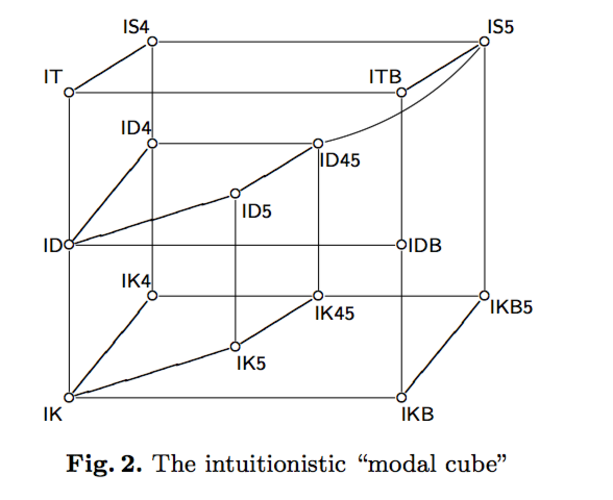
\includegraphics[width=1.5in]{intmodalcube.pdf}
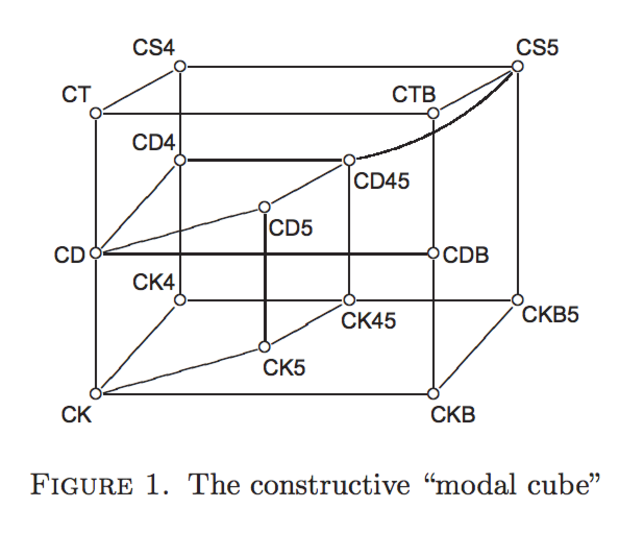
\includegraphics[width=1.6in]{constructivemodalcube.pdf}
%\caption{Modal Cubes}
\label{fig:modalcube}
\end{figure}

Sequent calculi  by themselves are not enough to provide us with Curry-Howard correspondences and/or term assignments for these systems. However, using the Prawitz S4 version of these modal systems we can easily produce a Curry-Howard correspondence and a categorical model for the Prawitz-style intuitionistic tense logic, our goal in this paper. 

We start by recalling the system using axioms, plain sequent calculus and plain natural deduction. In the next section we described a term assignment based on the dual calculus described in \cite{icalp1998} and show some of its syntactic prooperties. The next section  introduces the categorical model (a cartesian closed category with two intertwinned adjunctions) and show the usual soundness and completeness results. Finally we discuss potential applications and  limitations of our constructive tense logic.

\section{Tense Logic CS4-style}
We build up to the constructive tense logic we are interested in $\sf{TCS4}$ in progressive steps. We start with the intuitionistic basis $\sf{LJ}$, add the modalities to get the constructive S4 system, $\sf{CS4}$, provide the dual context modification (to help with the reuse of libraries, amongst other things), obtaining dual $\sf{CS4}$, $\sf{DCS4}$ and then finally consider the two adjunctions to obtain the tense constructive system $\sf{TCS4}$.


\subsection{Intuitionistic Sequent Calculus}
We start by recalling the basic sequent calculus for intuitionistic propositional logic, 
%Each of the logics presented in this section is an extension of the single-conclusion formalization of 
Gentzen's intuitionistic sequent calculus LJ.  
The syntax of formulas for LJ is defined by the
following grammar:
\begin{center}
    \begin{math}
        \begin{array}{lllllllll}
            A & ::= & p \mid \perp \mid A \land A \mid A \lor A \mid A \to B
        \end{array}
    \end{math}
\end{center}
The formula $p$ is taken from a set of countably many  propositional atoms. The constant $\top$ could be added, but it is the negation of the the falsum constant $\bot$.
%We begin with an initial set of inference rules, and then each system presented will be given as an extension of this initial system.  
The  initial inference rules, which just model
propositional intuitionistic logic, are as in 
Figure~\ref{fig:LJ}.

\begin{figure}
  \begin{mdframed}
\begin{center}
  \small
  \begin{math}
    \begin{array}{c}
      \begin{array}{cccccccc}
        \infer[\text{Id}]{\Delta,A \vdash A}{
          \,
        }
        & \quad &
        \infer[\text{Cut}]{\Gamma,\Delta \vdash C}{
          \Gamma \vdash B
          &
          B,\Delta \vdash C
        }
        & \quad & 
        \infer[\perp_{\mathcal{L}}]{\Gamma,\perp \; \vdash A}{
          \,
        }\\\\
        \infer[\lor_{\mathcal{L}}]{\Gamma,A \lor B \vdash C}{
          \Gamma,A \vdash C
          &
          \Gamma,B \vdash C
        }
        & \quad &
        \infer[\lor_{\mathcal{R}_1}]{\Gamma \vdash A \lor B}{
          \Gamma \vdash A
        }
        & \quad &
        \infer[\lor_{\mathcal{R}_2}]{\Gamma \vdash A \lor B}{
          \Gamma \vdash B
        }\\\\
        \infer[\land_{\mathcal{L}_1}]{\Gamma,A \land B \vdash C}{
          \Gamma,A \vdash C
        }
        & \quad &
        \infer[\land_{\mathcal{L}_2}]{\Gamma,A \land B \vdash C}{
          \Gamma,B \vdash C
        }
        & \quad &
        \infer[\land_{\mathcal{R}}]{\Gamma \vdash A \land B}{
          \Gamma \vdash A
          &
          \Gamma \vdash B
        }\\\\
        
      \end{array}
      \\
      \begin{array}{cccccccc}
        \infer[\to_{\mathcal{L}}]{\Gamma,A \to B \vdash C}{
          \Gamma \vdash A
          &
          \Gamma,B \vdash C
        }
        & \quad &
        \infer[\to_{\mathcal{R}}]{\Gamma \vdash A \to B}{
          \Gamma, A \vdash B
        }
      \end{array}        
    \end{array}
  \end{math}
\end{center}
 \end{mdframed}
  \caption{Intuitionistic Propositional  Calculus ({\sf{LJ}})}
  \label{fig:LJ}
\end{figure}

Sequents denoted $\Gamma \vdash C$ consist of a multiset of formulas, (written as either $\Gamma$, $\Delta$, or a numbered version of either), and a formula $C$. The intuitive meaning is that the conjunction of the formulas in $\Gamma$ entails the formula $C$. So far this is our intuitionistic basis.

\subsection{Constructive modal \sf{S4}} 
Next we recall the sequent calculus formalization of system CS4.  
%This formalization  was proposed by Bierman and de Paiva \cite{CS4} and initially  was called  IS4 (for Intuitionistic system S4). This system gives rise to a complete family of systems, which are alternative to Simpson's intuitionistic systems~\cite{simpson1994}.
%Simpson proposed in his thesis ~\cite{simpson1994}systems  of intuitonsitic modal logics, forming a framework starting from intuitionistic K. These  were also calledIK, IKT, IS4, IS5, etc, hence it made sense to call the family of systems originating with the S4 above, the family of constructive modal systems CS, and Bierman and de Paiva's system CS4.  This is for instance how new work, such as \cite{arisaka2015}, describes these systems.
%The system CS4 does not satisfy thesetraditional distributions that are basic to classical modal logic. Some philosophical significance can be attached to thisdistribution, or lack thereof, and we discuss it later. First wedefine the system.


\begin{figure}
  \begin{mdframed}
    \begin{center}
      \begin{math}
        \begin{array}{ccccc}              
          \infer[\Box_{\mathcal{L}}]{\Gamma, \Box A \vdash B}{
            \Gamma,A \vdash B
          }
          & \quad &
          \infer[\Box_{\mathcal{R}}]{\Box\Gamma,\Delta \vdash \Box A}{
            \Box \Gamma \vdash A
          }\\\\
          \infer[\Diamond_{\mathcal{L}}]{\Delta,\Box\Gamma,\Diamond A \vdash \Diamond B}{
            \Box\Gamma,A \vdash \Diamond B
          }
          & \quad &
          \infer[\Diamond_{\mathcal{R}}]{\Gamma \vdash \Diamond A}{
            \Gamma \vdash A
          }
        \end{array}        
      \end{math}
    \end{center}
  \end{mdframed}
  \caption{Constructive S4 modal rules ({\sf{CS4}})}
  \label{fig:CS4}
\end{figure}

  We recap the modality rules in Figure~\ref{fig:CS4}. These, in addition to the initial set of inference rules, define the sequent calculus for CS4. In Figure 3, we write $\Box \Gamma$ for the sequence of boxed formulas $\Box G_1, \Box G_2, \ldots, \Box G_k$ where $\Gamma$ is the set $G_1, G_2, \ldots,  G_k$.

Note that we do have right rules and left  rules for introducing the new modal operators $\Box$ (necessity) and $\Diamond$ (posssibility), but these rules are not as symmetric as the propositional ones. Most importantly, we have a local restriciton on the rule that introduces the $\Box$ operator: We can only introduce $\Box$ in the conclusion, if all the assumptions are already boxed. Also the rules for  the $\Diamond$ operator presuppose that you have already $\Box$ operators.
This system is indeed constructive, $\Box$ and $\Diamond$ are independent logical operators and  $\Box A$ is not logically equivalent to $\lnot \Diamond \lnot A$, nor is $\Diamond A$ logically equivalent to $\lnot \Box \lnot A$.


This system has a nice proof theory.
Bierman and de Paiva \cite{bierman2000} show that it has a Hilbert-style presentation,  a Natural Deduction presentation, as well as a sequent calculus presentation and these presentations are proved equivalent, that is, they prove the same theorems. The sequent calculus satisfies cut-elimination, an old result from Ohnishi and Matsumoto~\cite{ohnishi1957}, as well as the subformula property.
The Natural Deduction formulation has a colourful history: one of its distinct features is that it was described in Prawitz' seminal book in Natural Deduction \cite{prawitz1965},
hence it is  sometimes called Prawitz S4 intuitionistic  modal logic. Most interestingly the system has both Kripke and categorical semantics, described respectively in \cite{alechinaetal} and
\cite{bierman2000} as well as an independent mathematical semantics in terms of simplicial sets, described by Goubault-Larrecq~\cite{goubault-larrecq}. 
%, it has been used in several applications within programming
%language theory \todo{Add references for these applications}.
%Examples include \cite{hmm}.


\subsection{The dual context modal S4 calculus}
An equivalent (in terms of provability) but more type-theoretic system can be produced for the modal logic CS4. This is not so well-known, but this system can  be given a presentation in terms of a categorical adjunction, between two cartesian closed categories, as we will describe in the next section. This categorical presentation has been described  both in \cite{bierman2000} and in \cite{icalp1998}, in the former, this is called the \textbf{multi-context} formulation of CS4 and the
rules are given  in Figure~\ref{fig:DCS4}. (We prefer to call it the dual context sequent calculus.) Note that the rules are Natural Deduction rules, as it should be clear from the fact that they are introduction and elimination rules.

\begin{figure}
  \begin{mdframed}
    \begin{center}
      \begin{math}
        \begin{array}{ccccc}              
          \infer[\Box_{\mathcal{I}}]{\Gamma; \Delta \vdash \Box A}{
            \Gamma;\emptyset \vdash  A
          }
          & \quad &
          \infer[\Box_{\mathcal{E}}]{\Gamma;\Delta \vdash B}{\Gamma; \Delta \vdash \Box A \hspace{.1in}
            \Gamma, A;\Delta \vdash B
          }\\\\
          \infer[\Diamond_{\mathcal{I}}]{\Gamma;\Delta \vdash \Diamond A}{
            \Gamma;\Delta \vdash A
          }
          & \quad &
          \infer[\Diamond_{\mathcal{E}}]{\Gamma;\Delta \vdash \Diamond B}{
            \Gamma ;\Delta \vdash \Diamond A \hspace{.1in}\Gamma; A\vdash \Diamond B
          }
        \end{array}        
      \end{math}
    \end{center}
  \end{mdframed}
  \caption{The dual context modal calculus ({\sf{DCS4}})}
  \label{fig:DCS4}
\end{figure}

The main difference in the dual context formulation of CS4 is the fact that the context now has modal formulas and non-necessarily modal ones, separated by a semi-colon as in $\Gamma ; \Delta$. The difficult rule of $\Box$ introduction now insists that to introduce a necessity operator $\Box$ on a conclusion, we need to have  an empty context of non-modal assumptions. This corresponds to the traditional idea that to prove something is necessarily the case, all its assumptions have to be also necessary (or it has no assumptions whatsoever).

These rules have been shown by Benton \cite{benton1995} and Barber \cite{barber1997} to correspond to an adjunction of the categories, in the case where the basis is Linear Logic and the modalities correspond to the exponentials.  
Instead of Linear Logic, we deal with constructive modal logic and the adjunction is between functors corresponding to operators  $\Diamond \vdash \Box $.

\subsection{The tense CS4 calculus}
Finally to get to the tense logic which is the main aim of this note, we need two such adjunctions, but intertwined. This follows the pattern explained by Ewald~\cite{ewald1986}. Thus $\Diamond$ is left-adjoint to $\blacksquare$ and $\blacklozenge$ is left-adjoint to $\Box$, where we are writing $\blacksquare$ for the operator we called past universal $H$ before and $\Box$ for the future necessity operator $G$. The past existential $P$ is $\Diamond$ and the future existential is $\bLozenge$  or $F$.

A version of a  sequent calculus  system for this constructive tense logic is given by the rules in Figure \ref{fig:biCS4}.
This can be  transformed into Natural Deduction in the style of \cite{bierman2000} as shown in Figure \ref{fig:NDCS4}. The problem is that the last two adjunction rules in Figure \ref{fig:biCS4} (that relate the two sets of modalities) are extremely badly-behaved proof-theoretically (no cut-elimination and no subformula property even for cut-free proofs), as discussed in page 35 of the full report by Benton \cite{benton1995}. In fact they are the reason for moving to a dual context calculus, as explained in that paper and also  in Barber's work \cite{barber1997}. 

The  dual context systems, as described in Barber and Benton's work, are proved equivalent to the system with a single modality operator, either `$!$' or `$\Box$'. This is because in Intuitionistic Linear Logic one is not usually interested in either \textit{why not?} `$?$' or `$\Diamond$'. (In Classical Linear Logic the possibility modality is defined by negation of the necessity modality, so this extension is easier to make \cite{paykin2014}.) Given that our main goal is to discuss categorical semantics, which we can do easily for the necessity modalities, in this note we  consider only two necessity-like modalities $\Box$ and $\blacksquare$, to begin with.

We would like to have a natural deduction version of the tense calculus in dual context style. A dual context-style presentation of a single necessity modality has been presented in Figure~\ref{fig:DCS4}. Now we need to add another necessity-like modality and discuss their interaction.  A preliminary attempt at such calculus is given in Figure \ref{fig:ND2CS4}.

This corresponds to an intuitionistic tense logic obtained by extending IPL with two pairs of adjoint modalities $(\bLozenge, \Box)$ and $(\Diamond, \blacksquare)$, with no explicit relationship between
the modalities of the same colour, namely, $(\bLozenge, \blacksquare)$ and $(\Diamond,\Box)$. 

\begin{figure}
  \begin{mdframed}
    \begin{center}
      \begin{math}
        \begin{array}{cccccccc}              
          \infer[\Box_{\mathcal{L}}]{\Gamma, \Box A\vdash B}{
            \Gamma,  A \vdash B
          }
          & \quad &
          \infer[\Box_{\mathcal{R}}]{\Box\Gamma,\Delta \vdash \Box A}{
            \Box \Gamma \vdash A
          }\\\\
          \infer[\bLozenge_{\mathcal{L}}]{\Delta,\Box\Gamma,\bLozenge A \vdash \bLozenge B}{
            \Box\Gamma,A \vdash \bLozenge B
          }
          & \quad &
          \infer[\bLozenge_{\mathcal{R}}]{\Gamma \vdash \bLozenge A}{
            \Gamma \vdash A
         } \\\\
         \infer[\blacksquare_{\mathcal{L}}]{\Gamma, \blacksquare A \vdash B}{
            \Gamma,A \vdash B
          }
          & \quad &
          \infer[\blacksquare_{\mathcal{R}}]{\blacksquare\Gamma,\Delta \vdash \blacksquare A}{
            \blacksquare \Gamma \vdash A
          }\\\\
          \infer[\Diamond_{\mathcal{L}}]{\Delta,\blacksquare \Gamma,\Diamond A \vdash \Diamond B}{
            \blacksquare\Gamma,A \vdash \Diamond B
          }
          & \quad &
          \infer[\Diamond_{\mathcal{R}}]{\Gamma \vdash \Diamond A}{
            \Gamma \vdash A
         } \\\\
         \infer[adj1_{\mathcal{L}}]{\bLozenge A \vdash  B}{   A \vdash \Box B
          }
          & \quad &
          \infer[adj1_{\mathcal{R}}]{A \vdash \Box B}{
            \bLozenge A\vdash B
            }
         \\\\
         \infer[adj2_{\mathcal{L}}]{\Diamond A \vdash  B}{
            A \vdash \blacksquare B
          }
          & \quad &
         \infer[adj2_{\mathcal{R}}]{A \vdash \blacksquare B}{
            \Diamond A\vdash B
         }  
        \end{array}        
      \end{math}
    \end{center}
  \end{mdframed}
  \caption{Tense S4 sequent rules  ({\sf{biCS4}})}
  \label{fig:biCS4}
\end{figure}

\begin{figure}
  \begin{mdframed}
    \begin{mathpar}      
      \TLLdruleiXXCArleft{}  \and
      \TLLdruleiXXCArRight{} \and
      \TLLdruleiXXGRight{}   \and
      \TLLdrulelXXIArLeft{}  \and
      \TLLdrulelXXLArRight{} \and
      \TLLdrulelXXLArLeft{}  \and
      \TLLdrulelXXFRight{}   \and
      \TLLdrulelXXFLeft{}    \and
      \TLLdrulelXXGLeft{}    
    \end{mathpar}
  \end{mdframed}
  \caption{LNL sequent rules}
  \label{fig:LNL-seq-rules}
\end{figure}

\begin{figure}
  \begin{mdframed}
    \begin{center}
      \begin{math}
        \begin{array}{ccc}
          \begin{array}{ccccc}              
          \infer[\Box_{\mathcal{E}}]{\Gamma \vdash B}{
            \Gamma\vdash \Box B
          }
          & \quad &
          \infer[\Box_{\mathcal{I}}]{\Gamma\vdash \Box B}{
        \Gamma\vdash \Box A_1, \ldots ,  \Gamma\vdash  \Box A_k  \hspace{.1in} \Box A_1, \ldots \Box A_k \vdash B
          }\\\\
          
          & \quad &
          \infer[\bLozenge_{\mathcal{I}}]{\Gamma \vdash \bLozenge A}{
            \Gamma \vdash A
         } \\\\
         \infer[\blacksquare_{\mathcal{E}}]{\Gamma \vdash A}{
            \Gamma \vdash \blacksquare A
          }
          & \quad &
          \infer[\blacksquare_{\mathcal{I}}]{\Gamma\vdash \blacksquare B}{
        \Gamma\vdash \blacksquare A_1, \ldots ,  \Gamma\vdash  \blacksquare A_k  \hspace{.1in} \blacksquare A_1, \ldots \blacksquare A_k \vdash B
          }\\\\
          
          & \quad &
          \infer[\Diamond_{\mathcal{I}}]{\Gamma \vdash \Diamond A}{
            \Gamma \vdash A
         } \\\\
        \end{array} \\\\
        \infer[\bLozenge_{\mathcal{E}}]{\Gamma \vdash   \bLozenge C}{
            \Gamma\vdash \Box A_1\ldots \Gamma\vdash \Box A_k \hspace{.05in}\Gamma\vdash \bLozenge B \hspace{.1in}  \Box A_1\ldots\Box A_k, B\vdash \bLozenge C
          }\\\\
          \infer[\Diamond_{\mathcal{E}}]{\Gamma \vdash   \Diamond C}{
            \Gamma\vdash \blacksquare A_1\ldots \Gamma\vdash \blacksquare A_k \hspace{.05in}\Gamma\vdash \Diamond B \hspace{.1in}  \blacksquare A_1\ldots\blacksquare A_k, B\vdash \Diamond C
          }
%          \\\\
%         \begin{array}{ccc}
%            \infer[adj_{\mathcal{L}}]{\bLozenge A \vdash  B}{
%            A \vdash \Box B
%          }
%          & \quad &
%          \infer[adj_{\mathcal{R}}]{A \vdash \Box B}{
%            \bLozenge A\vdash B
%         }
%          \end{array} 
        \end{array}
      \end{math}
    \end{center}
  \end{mdframed}
  \caption{Tense  S4 rules ND first version ({\sf{NDCS4}})}
  \label{fig:NDCS4}
\end{figure}

\begin{figure}
  \begin{mdframed}
    \begin{center}
      \begin{math}
        \begin{array}{ccc}
 %         \begin{array}{ccccc}              
          \infer[\Box_{\mathcal{I}}]{\Gamma_1; \Delta \vdash \Box A}{
              \Gamma_1; \emptyset \vdash  A
            }
            & 
            \infer[\Box_{\mathcal{E}}]{\Gamma_1; \Delta \vdash B}{\Gamma_1;  \Delta \vdash \Box A \hspace{.1in}
              \Gamma_1;  A;\Delta \vdash B
            } \\\\
              \infer[\bLozenge_{\mathcal{I}}]{\Gamma \vdash \bLozenge A}{
            \Gamma \vdash A
         } &  \infer[\bLozenge_{\mathcal{E}}]{\Gamma_1; \Delta \vdash \bLozenge B}{
             \Gamma_1; \Delta \vdash \bLozenge A \hspace{.1in}\Gamma_1;  A\vdash \bLozenge B
            }
           \\\\
         \infer[\blacksquare_{\mathcal{I}}]{\Gamma; \emptyset  \vdash \blacksquare A}{
            \Gamma; \emptyset  \vdash  A
          } & 
         \infer[\blacksquare_{\mathcal{E}}]{\Gamma_1; \Delta \vdash B}{\Gamma_1;  \Delta \vdash \blacksquare A \hspace{.1in}
              \Gamma_1;  A;\Delta \vdash B
          }\\\\
          \infer[\Diamond_{\mathcal{I}}]{\Gamma \vdash \Diamond A}{
            \Gamma \vdash A
        } &
          \infer[\Diamond_{\mathcal{E}}]{\Gamma_1; \Delta \vdash \Diamond B}{
               \Gamma_1; \Delta \vdash \Diamond A \hspace{.1in}\Gamma_1; A\vdash \Diamond B
          }
%          \begin{array}{ccc}
%            \infer[adj_{\mathcal{L}}]{\bLozenge A \vdash  B}{
%            A \vdash \Box B
%          }
%          & \quad &
%          \infer[adj_{\mathcal{R}}]{A \vdash \Box B}{
%            \bLozenge A\vdash B
%         }
%         \end{array} 
        \end{array}
      \end{math}
    \end{center}
  \end{mdframed}
  \caption{biS4 rules, dual context   version ({\sf{ND2CS4}})}
  \label{fig:ND2CS4}
\end{figure}

\begin{figure}
  \begin{mdframed}
    \begin{center}
      \begin{math}
        \begin{array}{l}
          \begin{array}{ccccc}            
            \infer[\Box{\text{Id}}]{\Gamma_1; \Gamma_2, A;\Delta \vdash A}{}
            & \quad &
            \infer[\BBox{\text{Id}}]{\Gamma_1, A;\Gamma_2;\Delta \vdash A}{}
            \\\\
            \infer[\Box_{\mathcal{I}}]{\Gamma_1; \Gamma_2;\Delta \vdash \Box A}{
              \Gamma_1; \Gamma_2;\emptyset \vdash  A
            }            
            & \quad &
            \infer[\Box_{\mathcal{E}}]{\Gamma_1; \Gamma_2;\Delta \vdash B}{\Gamma_1; \Gamma_2; \Delta \vdash \Box A \hspace{.1in}
              \Gamma_1; \Gamma_2, A;\Delta \vdash B
            }\\\\            
             \infer[\bLozenge_{\mathcal{I}}]{\Gamma_1; \Gamma_2;\Delta \vdash \bLozenge A}{
               \Gamma_1; \Gamma_2;\Delta \vdash A
             }
             & \quad &          
             \infer[\bLozenge_{\mathcal{E}}]{\Gamma_1; \Gamma_2;\Delta \vdash \bLozenge B}{
               \Gamma_1; \Gamma_2 ;\Delta \vdash \bLozenge A \hspace{.1in}\Gamma_1; \Gamma_2; A\vdash \bLozenge B
             }                          
          \end{array}
          \\\\
          \begin{array}{ccccc}
            \infer[\blacksquare_{\mathcal{I}}]{\Gamma_1; \Gamma_2; \Delta \vdash \blacksquare A}{
              \Gamma_1; \Gamma_2;\emptyset \vdash  A
            }
            & \quad &
            \infer[\blacksquare_{\mathcal{E}}]{\Gamma_1; \Gamma_2;\Delta \vdash B}{\Gamma_1; \Gamma_2; \Delta \vdash \blacksquare A \hspace{.1in}
              \Gamma_1, A; \Gamma_2;\Delta \vdash B
            }
            \\\\
             \infer[\Diamond_{\mathcal{I}}]{\Gamma_1; \Gamma_2;\Delta \vdash \Diamond A}{
               \Gamma_1; \Gamma_2;\Delta \vdash A
             }
             & \quad &
             \infer[\bLozenge_{\mathcal{E}}]{\Gamma_1; \Gamma_2;\Delta \vdash \bLozenge B}{
               \Gamma_1; \Gamma_2 ;\Delta \vdash \bLozenge A \hspace{.1in}\Gamma_1; \Gamma_2; A\vdash \bLozenge B
             }
          \end{array}    
        \end{array}
      \end{math}
    \end{center}
  \end{mdframed}
  \caption{Dual context 2CS4 calculus ({\sf{TCS4}})}
  \label{fig:TCS4}
\end{figure}

\subsection{Axioms}
Axiom sets for the system $\sf{TCS4}$ are easier to provide. We need a set for the basic system intuitionistic logic $\sf{LJ}$,  any traditional set would do, plus the axioms for modalities, as well as the rules \textbf{modus ponens} and \textbf{necessitation} for the two necessity operators:
\begin{figure}
  \begin{mdframed}
    \begin{center}
      \begin{math}
        \begin{array}{ccccc}              
          \infer[\Box_{{Nec}}]{\Box A }{
           A 
          }
          & \quad &
          \infer[\blacksquare_{{Nec}}]{ \blacksquare A}{
             A
          }
        & \infer[\mathcal{MP}]{  B}{
           A\to B \hspace{.1in} A  
          }
        \end{array}        
      \end{math}
    \end{center}
  \end{mdframed}
  \caption{Axiomatic Rules}
  \label{fig:nec-rules}
\end{figure}

We have similar  axioms to Ewald's \cite{ewald1986}, except that the duality between necessity and possibility is not strict (Ewald's original axioms (7) and (7') in page 171 of  \cite{ewald1986} are not valid) and that the possibility modalities we deal with, do not distribute over disjunction (Ewald's axioms (4) and (4') are not valid). Also note we do have  introspection and reflexivity valid, which correspond to Ewald's axioms (12) and (12'), as well as (13) and (13').

We are interested in the term assignment system and its properties, as our aim is to use these as type systems for innovative programming languages. So we needed to provide the systematic work that shows basic properties of the type system $\sf{TCS4}$ we are interested in, this is what we do in the next section.

\begin{figure}
  \begin{mdframed}
  \begin{center}
    \begin{math}
      \begin{array}{lll}
        \mbox{propositional basic intuitionistic  axioms}\\\\
        \begin{array}{ccc}          
          \Box (A \to B) &\to &(\Box A \to \Box B)\\
          \Box (A \to B) &\to &(\bLozenge A\to \bLozenge B)\\
          (\Box A\to A) &\land &(A\to \bLozenge A)\\
          (\Box A\to \Box\Box A) &\land &(\bLozenge \bLozenge A \to \bLozenge A)\\
          \blacksquare (A \to B) &\to &(\blacksquare A \to \blacksquare B)\\
          \blacksquare (A \to B) &\to &(\Diamond A\to \Diamond B)\\
          (\blacksquare A\to A) &\land &(A\to \Diamond A)\\
          (\blacksquare A\to \blacksquare\blacksquare A) &\land &(\Diamond \Diamond A \to \Diamond A)\\
          \Diamond \blacksquare A\to A &\land &A\to \blacksquare\Diamond A\\
          \bLozenge\Box A\to A &\land &A\to \Box \bLozenge A\\
        \end{array}
      \end{array}
      \end{math}
  \end{center}
 \end{mdframed}
  \caption{Axioms for $\sf{TCS4}$}
  \label{axiomCS4}
\end{figure}

\section{Term Assignment}
\label{sec:term_assignment}

Given the Natural Deduction system presented in the previous section,
we simply follow the recipes described in \cite{barber1997} to produce
a term assignment for these four kinds of modal operators.

We start by giving a calculus for annotating natural deduction proofs
in our CS4 tense calculus with typed $\lambda$-calculus terms. The
annotations must be such that types correspond to modal propositions,
terms correspond to proofs and proof normalisation corresponds to term
reduction. The basic typying judgements of our CS4 tense calculus are
of the form $\Gamma  \TLLsym{;}  \Delta  \vdash  \TLLnt{t}  \TLLsym{:}  \TLLnt{A}$ where $\Gamma$ declares modal
variables, which may occurr arbitrarily in a term, while $\Delta$
declares intuitionistic variables that may not occurr in a subterm of
the form $\Box \, \TLLnt{t}$ or $\blacksquare \, \TLLnt{t}$.

The typing rules for basic propositional logic can be found in
Figure~\ref{fig:term-assignment-basic}, and the typing rules for the
TCS4 modalities are in Figure~\ref{fig:term-assignment-TCS4}.
Finally, the reduction relation consists of the $\beta$-reduction
rules defined in Figure~\ref{fig:reduction-TCS4}, and the commuting
conversions defined in Figure~\ref{fig:commuting-conv-TCS4}; we omit
congruence rules in the interest of space.
\begin{figure}
  \begin{mdframed}
    \begin{mathpar}
      \TLLdruletyXXax{} \and
      \TLLdruletyXXbax{} \and
      \TLLdruletyXXtrue{} \and
      \TLLdruletyXXfalse{} \and
      \TLLdruletyXXconjI{} \and
      \TLLdruletyXXconjEOne{} \and
      \TLLdruletyXXconjETwo{} \and
      \TLLdruletyXXdisjIOne{} \and
      \TLLdruletyXXdisjITwo{} \and
      \TLLdruletyXXdisjE{} \and
      \TLLdruletyXXimpI{} \and
      \TLLdruletyXXimpE{}      
    \end{mathpar}
  \end{mdframed}
  \caption{Term assignment for basic propositional logic}
  \label{fig:term-assignment-basic}
\end{figure}
\begin{figure}
  \begin{mdframed}
    \begin{mathpar}
      \TLLdruletyXXboxI{} \and
      \TLLdruletyXXboxE{} \and
      \TLLdruletyXXbdiaI{} \and
      \TLLdruletyXXbdiaE{} \and
      \TLLdruletyXXbboxI{} \and
      \TLLdruletyXXbboxE{} \and
      \TLLdruletyXXdiaI{} \and
      \TLLdruletyXXdiaE{}
    \end{mathpar}
  \end{mdframed}
  \caption{Term assignment for TCS4}
  \label{fig:term-assignment-TCS4}
\end{figure}
\begin{figure}
  \begin{mdframed}
    \begin{mathpar}
      \TLLdrulerXXbeta{} \and
      \TLLdrulerXXfirst{} \and
      \TLLdrulerXXsecond{} \and
      \TLLdrulerXXcaseOne{} \and
      \TLLdrulerXXcaseTwo{} \and
      \TLLdrulerXXbox{} \and
      \TLLdrulerXXbdia{} \and
      \TLLdrulerXXbbox{} \and
      \TLLdrulerXXdia{}      
    \end{mathpar}
  \end{mdframed}
  \caption{The $\beta$-reduction rules for TCS4}
  \label{fig:reduction-TCS4}
\end{figure}
\begin{figure}
  \begin{mdframed}
    \begin{mathpar}
      \TLLdrulerXXboxBox{} \and
      \TLLdrulerXXbdiaBdia{} \and
      \TLLdrulerXXboxBBox{} \and
      \TLLdrulerXXdiadia{}
    \end{mathpar}
  \end{mdframed}
  \caption{The commuting conversions for TCS4}
  \label{fig:commuting-conv-TCS4}
\end{figure}
In the remainder of this section we prove various properties of this
system.  TCS4 has two different types of assumptions, and hence, of
free variables, those that are members of $\Gamma$ and those that are
members of $\Delta$, where the former are implicitly boxed.  This
implies that there are two types of substitution for typing and
weakening results.
\begin{lemma}[Substitution for Typing]
  \label{lemma:substitution_for_typing}
  \begin{enumerate}[i.]
  \item[] 
  \item If $\Gamma  \TLLsym{;}  \Delta  \vdash  \TLLnt{t_{{\mathrm{1}}}}  \TLLsym{:}  \TLLnt{A}$, and $\Gamma  \TLLsym{,}  \mathit{x}  \TLLsym{:}  \TLLnt{A}  \TLLsym{;}  \Delta  \vdash  \TLLnt{t_{{\mathrm{2}}}}  \TLLsym{:}  \TLLnt{B}$, then $\Gamma  \TLLsym{;}  \Delta  \vdash  \TLLsym{[}  \TLLnt{t_{{\mathrm{1}}}}  \TLLsym{/}  \mathit{x}  \TLLsym{]}  \TLLnt{t_{{\mathrm{2}}}}  \TLLsym{:}  \TLLnt{B}$.
  \item If $\Gamma  \TLLsym{;}  \Delta  \vdash  \TLLnt{t_{{\mathrm{1}}}}  \TLLsym{:}  \TLLnt{A}$, and $\Gamma  \TLLsym{;}  \Delta  \TLLsym{,}  \mathit{x}  \TLLsym{:}  \TLLnt{A}  \vdash  \TLLnt{t_{{\mathrm{2}}}}  \TLLsym{:}  \TLLnt{B}$, then $\Gamma  \TLLsym{;}  \Delta  \vdash  \TLLsym{[}  \TLLnt{t_{{\mathrm{1}}}}  \TLLsym{/}  \mathit{x}  \TLLsym{]}  \TLLnt{t_{{\mathrm{2}}}}  \TLLsym{:}  \TLLnt{B}$.
  \end{enumerate}
\end{lemma}
\begin{proof}
  Both parts of this proof hold by straightforward induction on the
  form of the second assumed typing derivation.  Notice that rules
  $\Box_{\mathcal{I}}$ and $\BBox_{\mathcal{I}}$ do not need to be
  considered in in the proof of part two, because we assume the
  propositional context, $\Delta$, is non-empty.
\end{proof}

\begin{lemma}[Weakening]
  \label{lemma:weakening}
  \begin{enumerate}[i.]
  \item[]
  \item If $\Gamma  \TLLsym{;}  \Delta  \vdash  \TLLnt{t}  \TLLsym{:}  \TLLnt{B}$, then $\Gamma  \TLLsym{,}  \mathit{x}  \TLLsym{:}  \TLLnt{A}  \TLLsym{;}  \Delta  \vdash  \TLLnt{t}  \TLLsym{:}  \TLLnt{B}$.
  \item If $\Gamma  \TLLsym{;}  \Delta  \vdash  \TLLnt{t}  \TLLsym{:}  \TLLnt{B}$, then $\Gamma  \TLLsym{;}  \Delta  \TLLsym{,}  \mathit{x}  \TLLsym{:}  \TLLnt{A}  \vdash  \TLLnt{t}  \TLLsym{:}  \TLLnt{B}$.
  \end{enumerate}
\end{lemma}
\begin{proof}
  Both parts of this proof hold by straightforward induction on the
  form of the assumed typing derivation.  In the case of the rules
  $\Box_{\mathcal{I}}$ and $\BBox_{\mathcal{I}}$ we simply reapply the
  rule using the assumed premise.
\end{proof}


% section term_assignments (end)


\section{The Categorical Model}
There is not much essentially new in what we discuss here about the tense logic based on $\sf{CS4}$. Similar ideas were discussed by  Ghilardi and Meloni \cite{ghilardi1988}, Makkai and Reyes \cite{makkai1995} and more recently in by Dzik et al \cite{dziketal2012} and Menni and Smith \cite{Menni:2014}.

The upshot of our discussion is that the categorical model we advance is a cartesian closed category endowed with two adjunctions, corresponding to the (limited) universal and existential quantifications relative to the past and to the future that correspond to the two sets of  necessity and possibility operators.
%, relative to the past and the future.

This setting is though  different enough from the precursors we know about, to justify this note. First, as discussed elsewhere \cite{bierman2000}, we see no reason for the monads/comonads emerging from this setting to be \textbf{idempotent} operators, as they are in \cite{ghilardi1988} or \cite{makkai1995}. Secondly we see no reason to take our models as part of toposes, as we are not  interested in extra structure provided by toposes. 
However, we also see no reason to confine ourselves to algebraic models such as Heyting algebras with operators, as degenerate posetal categories, as both \cite{dziketal2012} and  \cite{Menni:2014} do. Different proofs of the same theorem are important to us as they correspond to different morphisms in the category between the same objects. Thus we are interested in \textbf{proof relevant} semantics, not simply provability.

We build our main definition in stages. A categorical model of propositional intuitionistic  logic is a \textbf{cartesian closed} category with coproducts $\cat{C}$.

\iffalse
\begin{definition}[modal S4 category]
  \label{def:CS4-model}
  Suppose $\cat{C}$ is a cartesian closed category equipped with  a monoidal comonad $(\Box, \varepsilon, \delta)$ and a
  \emph{$\Box$-strong monad} with a strength natural transformation
  \[
  \st{A}{B} : \Box A \pd \Diamond B \mto \Diamond(\Box A \pd B)
  \]
  This is a model of CS4 as defined and showed sound and complete in \cite{bierman2000}. We call this structure a \textit{$\sf{S4}$ modal category}.
  % as CS4 is the only kind of modality we consider in this note.
\end{definition}
\fi 

\begin{definition}[adjoint model]
  \label{def:CS4-single-adjoint-cat-model}
  An adjoint categorical model of dual context modal logic $\sf{DCS4}$ consists of the following data:
  \begin{enumerate}
  \item A cartesian closed category with coproducts $(\cat{C},1,0,\pd,+,\ihom)$;
  \item 
    A monoidal adjunction  $F \dashv G$, where $(F,m)$ and  $(G,n)\colon \cat{C} \mto \cat{C}$ are monoidal functors such that their composition $GF$ is a monoidal comonad, written as $\Box$;
 \item The  monad $(\Diamond, \eta, \mu, \st{A}{B})$, induced by the adjunction $F \dashv G$,   is $\Box$-strong.
  \end{enumerate}
\end{definition}

\iffalse
Define an interpretation $\sem{\_} : \sf{DCS4} \to {\cal C}$ which takes the types and sequents of $\sf{DCS4}$ (over a basic 
set of types)  to a model $\cal C$ as follows:
\begin{align*}
\sem{p} &= I(p) \mbox{  for $p$ a base type}\\
\sem{\top} &= \top\\
[A\times B] &= [A]\times [B]\\
\sem{  A \to B  } &=  \sem{ A}  \to  \sem{ B }\\
\sem{\Box A} &= F G(\sem{A})
\end{align*}
 Throughout this section we will denote the separation of contexts
 into two disjoint contexts as $[[G]] = [[G' | D]]$ where $[[G']]$
 contains modal assumptions We extend this interpretation to to lists of types by saying
 that for a list $A_1, ..., A_n$ of types, the interpretation of the
 list is the list of the interpretations $\sem{A_1,...A_n} =
 (\sem{A_1}, . . . \sem{A_n})$ contexts $(A_1,...A_n | \ B_1,...B_n)$
 by adding boxes to the modal assumptions and defining $
 \sem{A_1,\ldots, A_n |\ B_1,\ldots,B_n} = \Box \sem{A_1}\times \cdots
 \times \Box \sem{A_n} \times \ \sem{B_1}\times \cdots \times\sem{B_n}
 $.  The interpretation will take a sequent $\Gamma|\Delta \vdash t :
 A$ to an arrow $ \sem {\Gamma|\Delta \vdash t : A} : \sem{
   \Gamma|\Delta} \to \sem{A} $ in the adjoint modal category.

The $\sf{DCS4}$ type theory can be soundly interpreted in an adjoint modal category as defined above.
\begin{theorem}
\label{thm:dcs4-sound}
The type theory $\sf{DCS4}$  has  \textit{sound} models provided by the structures $\cal C$ defined above.
In other words, given an adjoint modal category $\cal C$, using the above interpretation, the following hold:
\begin{itemize}
\item Assume $\Gamma|\Delta \vdash t : A$ in $\sf{DCS4}$. Then $\sem{\Gamma |
    \Delta \vdash t \colon A}$ is a morphism  with domain
  $\sem{\Gamma | \Delta}$ and codomain $\sem{A}$;
\item Assume $\Gamma \vdash t = s \colon A$. Then $\sem{\Gamma
  \vdash t \colon A} = \sem{\Gamma \vdash s \colon A}$.
\end{itemize}
\end{theorem}

We also have completeness of adjoint modal categories:
\begin{theorem}
\label{thm:diml-completeness}
The adjoint modal models are \textit{complete} in the appropriate sense for the type theory $\sf{DCS4}$. This is to say, if
we have equality of the interpretations $\sem{\Gamma \vdash t \colon A} = \sem{\Gamma  \vdash s \colon A}$
 (where \mbox{$\sem{\ } $} is the interpretation defined above)
 in the
adjoint modal category $\cal C$
   for any derived sequents $\Gamma \vdash t \colon A$
 and $\Gamma \vdash s \colon A$ 
 then we can derive the  equation in the type theory $\sf{DCS4}$ $\;$
 $\Gamma \vdash t = s \colon A$. 
\end{theorem}

The proof is usual: we construct the term model and show that the basic rules of the calculus are mapped to 
appropriate morphisms using  the categorical constructs. 
\fi 

\begin{definition}[tense calculus model]
A model of $\sf{TCDS4}$ is a cartesian closed category $\cal{C}$ as above, together with two intertwined adjunctions $(\bLozenge\dashv \Box, \Diamond\dashv \blacksquare)$.  The adjunctions $(\bLozenge\dashv \Box)$ and $(\Diamond\dashv \blacksquare)$ on $\cal{C}$ are connected by Fisher-Servi axioms. 
\end{definition}

Categorical soundness is proved, as usual, checking the natural deduction rules preserve validity of the constructions used, i.e function spaces, products, coproducts and the two adjunctions. 

Define an interpretation $\sem{\_} : \sf{TCS4} \to {\cal C}$ which takes the types and sequents of $\sf{TCS4}$ (over a basic 
set of types)  to a model $\cal C$ as follows:
\begin{align*}
\sem{p} &= I(p) \mbox{  for $p$ a base type}\\
\sem{\top} &= \top\\
[A\times B] &= [A]\times [B]\\
\sem{  A \to B  } &=  \sem{ A}  \to  \sem{ B }\\
\sem{\Box A} &= F G(\sem{A})\\
\sem{\blacksquare A} &= F' G'(\sem{A})
\end{align*}
 We extend this interpretation to 
 to lists of types by saying that for a list $A_1, ..., A_n$ of types,
 the interpretation of the list is the list of the interpretations
 $\sem{A_1,...A_n} = (\sem{A_1}, . . . \sem{A_n})$ 
 %Secondly, we extend the definition to contexts
contexts $(A_1,...A_n | \ B_1,...B_n)$ by adding (two kinds of) boxes to the modal
assumptions and defining
$ \sem{A_1,\ldots, A_n |\  B_1,\ldots,B_n} = 
\Box \sem{A_1}\times \cdots \times \Box \sem{A_n} \times
\  \sem{B_1}\times \cdots \times\sem{B_n} $.
The interpretation will take a sequent $\Gamma|\Delta \vdash t : A$ to an arrow 
$ \sem {\Gamma|\Delta \vdash t : A} : \sem{ \Gamma|\Delta} \to \sem{A} $
in the tense modal category.


\begin{theorem}
\label{thm:tcs4-csound}
The type theory $\sf{TCS4}$  has  \textit{sound} models provided by the structures $\cal C$ defined above.
In other words, given an tense adjoint modal category $\cal C$, using the above interpretation, the following hold:
\begin{itemize}
\item Assume $\Gamma|\Delta \vdash t : A$ in $\sf{TCS4}$. Then $\sem{\Gamma |
    \Delta \vdash t \colon A}$ is a morphism  with domain
  $\sem{\Gamma | \Delta}$ and codomain $\sem{A}$;
\item Assume $\Gamma \vdash t = s \colon A$. Then $\sem{\Gamma
  \vdash t \colon A} = \sem{\Gamma \vdash s \colon A}$.
\end{itemize}
\end{theorem}



We also have completeness of the tense modal categories.

\begin{theorem}
\label{thm:tcs4-completeness}
The adjoint modal models are \textit{complete} in the appropriate sense for the type theory $\sf{TCS4}$. This is to say, if
we have equality of the interpretations $\sem{\Gamma \vdash t \colon A} = \sem{\Gamma  \vdash s \colon A}$
 (where \mbox{$\sem{\ } $} is the interpretation defined above)
 in the
tense modal category $\cal C$
   for any derived sequents $\Gamma \vdash t \colon A$
 and $\Gamma \vdash s \colon A$ 
 then we can derive the  equation in the type theory $\sf{TCS4}$ $\;$
 $\Gamma \vdash t = s \colon A$. 
\end{theorem}
Categorical completeness requires providing an equivalence relation in the Lindenbaum algebra of the formulae, as usual in algebraic semantics. The basic calculations, for traditional algebraic semantics in Heyting algebras were provided, for instance, by Figallo et al in \cite{figallo2014}. \textit{Mutatis mutantis} these calculations will apply for our version of the system (no distribution of diamonds over disjunctions, no definibility of diamonds in terms of negated boxes).
%\section{Applications}

\section{Conclusions}
We have described a tense version of constructive temporal logic, conceived as a basic category of propositions, together with two adjunctions, corresponding to two kinds of  necessity 
%and possibility 
modalities, in the future and in the past. This system is based on traditional work of Ewald in \cite{ewald1986}, where we simply do the modifications required to account for the  categorical model desired. This work is somewhat inspired by recent work on Functional Reactive Programming (FRP) by Jeltsch \cite{jeltsch2012} and Jeffrey \cite{jeffrey2012}, independently. Both of these works consider Curry-Howard correspondents to temporal logic, but they tend to concentrate on the \textit{next} temporal operator, originally considered in LTL (Linear Temporal Logic) as suggested by Davies. The temporal operators we consider are more abstract and one can hope that they may shed some light on the issues of FRP. But this is future work.

\bibliographystyle{plain}
\bibliography{references}

\appendix

\section{Appendix}
\label{sec:appendix}

\subsection{Proofs}
\label{subsec:proofs}
\subsubsection{Proof of Substitution for Typing}
\label{sec:proof_of_lemma:substitution_for_typing}

\begin{lemma*}[Substitution for Typing]
  If $\Gamma_{{\mathrm{1}}}  \vdash  \TLLnt{t_{{\mathrm{1}}}}  \TLLsym{:}  \TLLnt{A}$, and $\Gamma_{{\mathrm{1}}}  \TLLsym{,}  \mathit{x}  \TLLsym{:}  \TLLnt{A}  \TLLsym{,}  \Gamma_{{\mathrm{2}}}  \vdash  \TLLnt{t_{{\mathrm{2}}}}  \TLLsym{:}  \TLLnt{B}$, then $\Gamma_{{\mathrm{1}}}  \TLLsym{,}  \Gamma_{{\mathrm{2}}}  \vdash  \TLLsym{[}  \TLLnt{t_{{\mathrm{1}}}}  \TLLsym{/}  \mathit{x}  \TLLsym{]}  \TLLnt{t_{{\mathrm{2}}}}  \TLLsym{:}  \TLLnt{B}$.
\end{lemma*}

\begin{proof}
  Suppose $\Gamma_{{\mathrm{1}}}  \vdash  \TLLnt{t_{{\mathrm{1}}}}  \TLLsym{:}  \TLLnt{A}$ and $\Gamma_{{\mathrm{1}}}  \TLLsym{,}  \mathit{x}  \TLLsym{:}  \TLLnt{A}  \TLLsym{,}  \Gamma_{{\mathrm{2}}}  \vdash  \TLLnt{t_{{\mathrm{2}}}}  \TLLsym{:}  \TLLnt{B}$.  We case
split on the structure of the latter.
\begin{itemize}
\item[] Case.\\ 
  \begin{center}
    \begin{math}
      $$\mprset{flushleft}
      \inferrule* [right=$\text{Id}$] {
        \ 
      }{\Gamma_{{\mathrm{1}}}  \TLLsym{,}  \mathit{x}  \TLLsym{:}  \TLLnt{A}  \TLLsym{,}  \Gamma_{{\mathrm{2}}}  \vdash  \mathit{y}  \TLLsym{:}  \TLLnt{C}}
    \end{math}
  \end{center}
  In this case $\TLLnt{t_{{\mathrm{2}}}} = \mathit{y}$ and $\TLLnt{B} = \TLLnt{C}$.  We are not
  sure if $\mathit{x} = \mathit{y}$, thus, we must consider the case when they
  are and are not equal.

  Suppose $\mathit{x} \neq \mathit{y}$.  Then $\TLLsym{[}  \TLLnt{t_{{\mathrm{1}}}}  \TLLsym{/}  \mathit{x}  \TLLsym{]}  \TLLnt{t_{{\mathrm{2}}}} = \TLLsym{[}  \TLLnt{t_{{\mathrm{1}}}}  \TLLsym{/}  \mathit{x}  \TLLsym{]}  \mathit{y} =
  \mathit{y}$ by the definition of substitution.  In addition, it must be
  the case that either $\mathit{y}  \TLLsym{:}  \TLLnt{C} \in \Gamma_{{\mathrm{1}}}$ or $\mathit{y}  \TLLsym{:}  \TLLnt{C} \in
  \Gamma_{{\mathrm{2}}}$.  This implies that $\Gamma_{{\mathrm{1}}}  \TLLsym{,}  \Gamma_{{\mathrm{2}}}  \vdash  \mathit{y}  \TLLsym{:}  \TLLnt{C}$ or $\Gamma_{{\mathrm{1}}}  \TLLsym{,}  \Gamma_{{\mathrm{2}}}  \vdash  \TLLsym{[}  \TLLnt{t_{{\mathrm{1}}}}  \TLLsym{/}  \mathit{x}  \TLLsym{]}  \TLLnt{t_{{\mathrm{2}}}}  \TLLsym{:}  \TLLnt{B}$ hold.

  Now suppose $\mathit{x} = \mathit{y}$.  Then $\TLLnt{A} = \TLLnt{B}$, and $\TLLsym{[}  \TLLnt{t_{{\mathrm{1}}}}  \TLLsym{/}  \mathit{x}  \TLLsym{]}  \TLLnt{t_{{\mathrm{2}}}} = \TLLsym{[}  \TLLnt{t_{{\mathrm{1}}}}  \TLLsym{/}  \mathit{x}  \TLLsym{]}  \mathit{x} = \TLLnt{t_{{\mathrm{1}}}}$ by the definition of
  substitution.  Thus, $\Gamma_{{\mathrm{1}}}  \TLLsym{,}  \Gamma_{{\mathrm{2}}}  \vdash  \TLLsym{[}  \TLLnt{t_{{\mathrm{1}}}}  \TLLsym{/}  \mathit{x}  \TLLsym{]}  \TLLnt{t_{{\mathrm{2}}}}  \TLLsym{:}  \TLLnt{B}$ holds, because we
  know $\Gamma_{{\mathrm{1}}}  \TLLsym{,}  \Gamma_{{\mathrm{2}}}  \vdash  \TLLnt{t_{{\mathrm{1}}}}  \TLLsym{:}  \TLLnt{A}$.

\item[] Case.\\ 
  \begin{center}
    \begin{math}
      $$\mprset{flushleft}
      \inferrule* [right=$\perp_\mathcal{E}$] {
        \ 
      }{\Gamma_{{\mathrm{1}}}  \TLLsym{,}  \mathit{x}  \TLLsym{:}  \TLLnt{A}  \TLLsym{,}  \Gamma_{{\mathrm{2}}}  \TLLsym{,}  \mathit{y}  \TLLsym{:}  \perp  \vdash   \mathsf{contra}   \TLLsym{:}  \TLLnt{C}}
    \end{math}
  \end{center}
  We must show that $\Gamma_{{\mathrm{1}}}  \TLLsym{,}  \Gamma_{{\mathrm{2}}}  \TLLsym{,}  \mathit{y}  \TLLsym{:}  \perp  \vdash  \TLLsym{[}  \TLLnt{t_{{\mathrm{1}}}}  \TLLsym{/}  \mathit{x}  \TLLsym{]}   \mathsf{contra}   \TLLsym{:}  \TLLnt{C}$ holds,
  because $\TLLnt{B} = \TLLnt{C}$ and $\TLLnt{t_{{\mathrm{2}}}} =  \mathsf{contra} $, but this holds
  by reapplying the rule.


\item[] Case.\\ 
  \begin{center}
    \begin{math}
      $$\mprset{flushleft}
      \inferrule* [right=$\TLLdruletyXXimpIName$] {
        \Gamma_{{\mathrm{1}}}  \TLLsym{,}  \mathit{x}  \TLLsym{:}  \TLLnt{A}  \TLLsym{,}  \Gamma_{{\mathrm{2}}}  \TLLsym{,}  \mathit{y}  \TLLsym{:}  \TLLnt{C_{{\mathrm{1}}}}  \vdash  \TLLnt{t}  \TLLsym{:}  \TLLnt{C_{{\mathrm{2}}}}
      }{\Gamma_{{\mathrm{1}}}  \TLLsym{,}  \mathit{x}  \TLLsym{:}  \TLLnt{A}  \TLLsym{,}  \Gamma_{{\mathrm{2}}}  \vdash   \lambda  \mathit{y}  :  \TLLnt{C_{{\mathrm{1}}}} . \TLLnt{t}   \TLLsym{:}  \TLLnt{C_{{\mathrm{1}}}}  \to  \TLLnt{C_{{\mathrm{2}}}}}
    \end{math}
  \end{center}
  In this case $\TLLnt{B} = \TLLnt{C_{{\mathrm{1}}}}  \to  \TLLnt{C_{{\mathrm{2}}}}$ and $\TLLnt{t_{{\mathrm{2}}}} =  \lambda  \mathit{y}  :  \TLLnt{C} . \TLLnt{t} $.  By the induction hypothesis
  we know $\Gamma_{{\mathrm{1}}}  \TLLsym{,}  \Gamma_{{\mathrm{2}}}  \TLLsym{,}  \mathit{y}  \TLLsym{:}  \TLLnt{C_{{\mathrm{1}}}}  \vdash  \TLLsym{[}  \TLLnt{t_{{\mathrm{1}}}}  \TLLsym{/}  \mathit{x}  \TLLsym{]}  \TLLnt{t}  \TLLsym{:}  \TLLnt{C_{{\mathrm{2}}}}$, and then by reapplying the rule we know
  $\Gamma_{{\mathrm{1}}}  \TLLsym{,}  \Gamma_{{\mathrm{2}}}  \vdash   \lambda  \mathit{y}  :  \TLLnt{C_{{\mathrm{1}}}} . \TLLsym{[}  \TLLnt{t_{{\mathrm{1}}}}  \TLLsym{/}  \mathit{x}  \TLLsym{]}  \TLLnt{t}   \TLLsym{:}  \TLLnt{C_{{\mathrm{2}}}}$ holds.  However, by the definition of substitution
  we know $ \lambda  \mathit{y}  :  \TLLnt{C_{{\mathrm{1}}}} . \TLLsym{[}  \TLLnt{t_{{\mathrm{1}}}}  \TLLsym{/}  \mathit{x}  \TLLsym{]}  \TLLnt{t}  = \TLLsym{[}  \TLLnt{t_{{\mathrm{1}}}}  \TLLsym{/}  \mathit{x}  \TLLsym{]}  \TLLsym{(}   \lambda  \mathit{y}  :  \TLLnt{C_{{\mathrm{1}}}} . \TLLnt{t}   \TLLsym{)}$, and thus, we obtain our result.

\item[] Case.\\ 
  \begin{center}
    \begin{math}
      $$\mprset{flushleft}
      \inferrule* [right=$\TLLdruletyXXimpEName$] {
        \Gamma_{{\mathrm{1}}}  \TLLsym{,}  \mathit{x}  \TLLsym{:}  \TLLnt{A}  \TLLsym{,}  \Gamma_{{\mathrm{2}}}  \vdash  \TLLnt{t'_{{\mathrm{1}}}}  \TLLsym{:}  \TLLnt{C_{{\mathrm{1}}}}  \to  \TLLnt{C_{{\mathrm{2}}}}  \quad  \Gamma_{{\mathrm{1}}}  \TLLsym{,}  \mathit{x}  \TLLsym{:}  \TLLnt{A}  \TLLsym{,}  \Gamma_{{\mathrm{2}}}  \vdash  \TLLnt{t'_{{\mathrm{2}}}}  \TLLsym{:}  \TLLnt{C_{{\mathrm{1}}}}
      }{\Gamma_{{\mathrm{1}}}  \TLLsym{,}  \mathit{x}  \TLLsym{:}  \TLLnt{A}  \TLLsym{,}  \Gamma_{{\mathrm{2}}}  \vdash  \TLLnt{t'_{{\mathrm{1}}}} \, \TLLnt{t'_{{\mathrm{2}}}}  \TLLsym{:}  \TLLnt{C_{{\mathrm{2}}}}}
    \end{math}
  \end{center}
  We now have that $\TLLnt{B} = \TLLnt{C_{{\mathrm{2}}}}$ and $\TLLnt{t_{{\mathrm{2}}}} = \TLLnt{t'_{{\mathrm{1}}}} \, \TLLnt{t'_{{\mathrm{2}}}}$.  By the induction hypothesis
  we know that $\Gamma_{{\mathrm{1}}}  \TLLsym{,}  \Gamma_{{\mathrm{2}}}  \vdash  \TLLsym{[}  \TLLnt{t_{{\mathrm{1}}}}  \TLLsym{/}  \mathit{x}  \TLLsym{]}  \TLLnt{t'_{{\mathrm{1}}}}  \TLLsym{:}  \TLLnt{C_{{\mathrm{1}}}}  \to  \TLLnt{C_{{\mathrm{2}}}}$ and $\Gamma_{{\mathrm{1}}}  \TLLsym{,}  \Gamma_{{\mathrm{2}}}  \vdash  \TLLsym{[}  \TLLnt{t_{{\mathrm{1}}}}  \TLLsym{/}  \mathit{x}  \TLLsym{]}  \TLLnt{t'_{{\mathrm{2}}}}  \TLLsym{:}  \TLLnt{C_{{\mathrm{1}}}}$ both hold.
  Then by reapplying the rule we obtain that $\Gamma_{{\mathrm{1}}}  \TLLsym{,}  \Gamma_{{\mathrm{2}}}  \vdash  \TLLsym{(}  \TLLsym{[}  \TLLnt{t_{{\mathrm{1}}}}  \TLLsym{/}  \mathit{x}  \TLLsym{]}  \TLLnt{t'_{{\mathrm{1}}}}  \TLLsym{)} \, \TLLsym{(}  \TLLsym{[}  \TLLnt{t_{{\mathrm{1}}}}  \TLLsym{/}  \mathit{x}  \TLLsym{]}  \TLLnt{t'_{{\mathrm{2}}}}  \TLLsym{)}  \TLLsym{:}  \TLLnt{C_{{\mathrm{2}}}}$, and thus,
  by the definition of substitution $\Gamma_{{\mathrm{1}}}  \TLLsym{,}  \Gamma_{{\mathrm{2}}}  \vdash  \TLLsym{[}  \TLLnt{t_{{\mathrm{1}}}}  \TLLsym{/}  \mathit{x}  \TLLsym{]}  \TLLsym{(}  \TLLnt{t'_{{\mathrm{1}}}} \, \TLLnt{t'_{{\mathrm{2}}}}  \TLLsym{)}  \TLLsym{:}  \TLLnt{C_{{\mathrm{2}}}}$ holds.
  
  
\item[] Case.\\ 
  \begin{center}
    \scriptsize
    \begin{math}
      $$\mprset{flushleft}
      \inferrule* [right=$\TLLdruletyXXboxIName$] {
         \Gamma_{{\mathrm{1}}}  \TLLsym{,}  \mathit{x}  \TLLsym{:}  \TLLnt{A}  \TLLsym{,}  \Gamma_{{\mathrm{2}}}  \vdash  \TLLnt{t'_{{\mathrm{1}}}}  \TLLsym{:}  \Box \, \TLLnt{C_{{\mathrm{1}}}}  \TLLsym{,} \, ... \, \TLLsym{,}  \Gamma_{{\mathrm{1}}}  \TLLsym{,}  \mathit{x}  \TLLsym{:}  \TLLnt{A}  \TLLsym{,}  \Gamma_{{\mathrm{2}}}  \vdash  \TLLnt{t'_{\TLLmv{k}}}  \TLLsym{:}  \Box \, \TLLnt{C_{\TLLmv{k}}}   \quad  \mathit{x_{{\mathrm{1}}}}  \TLLsym{:}  \Box \, \TLLnt{C_{{\mathrm{1}}}}  \TLLsym{,} \, ... \, \TLLsym{,}  \mathit{x_{\TLLmv{k}}}  \TLLsym{:}  \Box \, \TLLnt{C_{\TLLmv{k}}}  \vdash  \TLLnt{t}  \TLLsym{:}  \TLLnt{C}
      }{\Gamma_{{\mathrm{1}}}  \TLLsym{,}  \mathit{x}  \TLLsym{:}  \TLLnt{A}  \TLLsym{,}  \Gamma_{{\mathrm{2}}}  \vdash   \mathsf{let}_\Box\, \mathit{x_{{\mathrm{1}}}}  \TLLsym{:}  \Box \, \TLLnt{C_{{\mathrm{1}}}}  \TLLsym{,} \, ... \, \TLLsym{,}  \mathit{x_{\TLLmv{k}}}  \TLLsym{:}  \Box \, \TLLnt{C_{\TLLmv{k}}} \,\mathsf{be}\, \TLLnt{t'_{{\mathrm{1}}}}  \TLLsym{,} \, ... \, \TLLsym{,}  \TLLnt{t'_{\TLLmv{k}}} \,\mathsf{in}\, \TLLnt{t}   \TLLsym{:}  \Box \, \TLLnt{C}}
    \end{math}
  \end{center}
  In this case $\TLLnt{B} = \Box \, \TLLnt{C}$ and
  $\TLLnt{t_{{\mathrm{2}}}} =  \mathsf{let}_\Box\, \mathit{x_{{\mathrm{1}}}}  \TLLsym{:}  \Box \, \TLLnt{C_{{\mathrm{1}}}}  \TLLsym{,} \, ... \, \TLLsym{,}  \mathit{x_{\TLLmv{k}}}  \TLLsym{:}  \Box \, \TLLnt{C_{\TLLmv{k}}} \,\mathsf{be}\, \TLLnt{t'_{{\mathrm{1}}}}  \TLLsym{,} \, ... \, \TLLsym{,}  \TLLnt{t'_{\TLLmv{k}}} \,\mathsf{in}\, \TLLnt{t} $.  By the induction hypothesis
  we know that 
  \[ \Gamma_{{\mathrm{1}}}  \TLLsym{,}  \Gamma_{{\mathrm{2}}}  \vdash  \TLLsym{[}  \TLLnt{t_{{\mathrm{1}}}}  \TLLsym{/}  \mathit{x}  \TLLsym{]}  \TLLnt{t'_{{\mathrm{1}}}}  \TLLsym{:}  \Box \, \TLLnt{C_{{\mathrm{1}}}} , \ldots , \Gamma_{{\mathrm{1}}}  \TLLsym{,}  \mathit{x}  \TLLsym{:}  \TLLnt{A}  \TLLsym{,}  \Gamma_{{\mathrm{2}}}  \vdash  \TLLsym{[}  \TLLnt{t_{{\mathrm{1}}}}  \TLLsym{/}  \mathit{x}  \TLLsym{]}  \TLLnt{t'_{\TLLmv{k}}}  \TLLsym{:}  \Box \, \TLLnt{C_{\TLLmv{k}}} \] all hold. Then by reapplying
  the rule we know that
  \[ \Gamma_{{\mathrm{1}}}  \TLLsym{,}  \Gamma_{{\mathrm{2}}}  \vdash   \mathsf{let}_\Box\, \mathit{x_{{\mathrm{1}}}}  \TLLsym{:}  \Box \, \TLLnt{C_{{\mathrm{1}}}}  \TLLsym{,} \, ... \, \TLLsym{,}  \mathit{x_{\TLLmv{k}}}  \TLLsym{:}  \Box \, \TLLnt{C_{\TLLmv{k}}} \,\mathsf{be}\, \TLLsym{[}  \TLLnt{t_{{\mathrm{1}}}}  \TLLsym{/}  \mathit{x}  \TLLsym{]}  \TLLnt{t'_{{\mathrm{1}}}}  \TLLsym{,} \, ... \, \TLLsym{,}  \TLLsym{[}  \TLLnt{t_{{\mathrm{1}}}}  \TLLsym{/}  \mathit{x}  \TLLsym{]}  \TLLnt{t'_{\TLLmv{k}}} \,\mathsf{in}\, \TLLnt{t}   \TLLsym{:}  \Box \, \TLLnt{C}, \] but by the definition
  of substitution and the fact that $\TLLsym{[}  \TLLnt{t_{{\mathrm{1}}}}  \TLLsym{/}  \mathit{x}  \TLLsym{]}  \TLLnt{t} = \TLLnt{t}$ because $\TLLnt{t}$ does not depend on $\mathit{x}$ we know that
  \[ \Gamma_{{\mathrm{1}}}  \TLLsym{,}  \Gamma_{{\mathrm{2}}}  \vdash  \TLLsym{[}  \TLLnt{t_{{\mathrm{1}}}}  \TLLsym{/}  \mathit{x}  \TLLsym{]}  \TLLsym{(}   \mathsf{let}_\Box\, \mathit{x_{{\mathrm{1}}}}  \TLLsym{:}  \Box \, \TLLnt{C_{{\mathrm{1}}}}  \TLLsym{,} \, ... \, \TLLsym{,}  \mathit{x_{\TLLmv{k}}}  \TLLsym{:}  \Box \, \TLLnt{C_{\TLLmv{k}}} \,\mathsf{be}\, \TLLnt{t'_{{\mathrm{1}}}}  \TLLsym{,} \, ... \, \TLLsym{,}  \TLLnt{t'_{\TLLmv{k}}} \,\mathsf{in}\, \TLLnt{t}   \TLLsym{)}  \TLLsym{:}  \Box \, \TLLnt{C} \] holds.
  
\item[] Case.\\ 
  \begin{center}
    \begin{math}
      $$\mprset{flushleft}
      \inferrule* [right=$\TLLdruletyXXboxEName$] {
        \Gamma_{{\mathrm{1}}}  \TLLsym{,}  \mathit{x}  \TLLsym{:}  \TLLnt{A}  \TLLsym{,}  \Gamma_{{\mathrm{2}}}  \vdash  \TLLnt{t}  \TLLsym{:}  \Box \, \TLLnt{C}
      }{\Gamma_{{\mathrm{1}}}  \TLLsym{,}  \mathit{x}  \TLLsym{:}  \TLLnt{A}  \TLLsym{,}  \Gamma_{{\mathrm{2}}}  \vdash  \mathsf{unbox}_\Box\, \, \TLLnt{t}  \TLLsym{:}  \TLLnt{C}}
    \end{math}
  \end{center}
  This case easily follows by first applying the induction hypothesis and reapplying the rule.

\item[] Case.\\ 
  \begin{center}
    \scriptsize
    \begin{math}
      $$\mprset{flushleft}
      \inferrule* [right=$\TLLdruletyXXbboxIName$] {
         \Gamma_{{\mathrm{1}}}  \TLLsym{,}  \mathit{x}  \TLLsym{:}  \TLLnt{A}  \TLLsym{,}  \Gamma_{{\mathrm{2}}}  \vdash  \TLLnt{t_{{\mathrm{1}}}}  \TLLsym{:}  \blacksquare \, \TLLnt{C_{{\mathrm{1}}}}  \TLLsym{,} \, ... \, \TLLsym{,}  \Gamma_{{\mathrm{1}}}  \TLLsym{,}  \mathit{x}  \TLLsym{:}  \TLLnt{A}  \TLLsym{,}  \Gamma_{{\mathrm{2}}}  \vdash  \TLLnt{t_{\TLLmv{k}}}  \TLLsym{:}  \blacksquare \, \TLLnt{C_{\TLLmv{k}}}   \quad  \mathit{x_{{\mathrm{1}}}}  \TLLsym{:}  \blacksquare \, \TLLnt{C_{{\mathrm{1}}}}  \TLLsym{,} \, ... \, \TLLsym{,}  \mathit{x_{\TLLmv{k}}}  \TLLsym{:}  \blacksquare \, \TLLnt{C_{\TLLmv{k}}}  \vdash  \TLLnt{t}  \TLLsym{:}  \TLLnt{C}
      }{\Gamma_{{\mathrm{1}}}  \TLLsym{,}  \mathit{x}  \TLLsym{:}  \TLLnt{A}  \TLLsym{,}  \Gamma_{{\mathrm{2}}}  \vdash   \mathsf{let}_\blacksquare\, \mathit{x_{{\mathrm{1}}}}  \TLLsym{:}  \blacksquare \, \TLLnt{C_{{\mathrm{1}}}}  \TLLsym{,} \, ... \, \TLLsym{,}  \mathit{x_{\TLLmv{k}}}  \TLLsym{:}  \blacksquare \, \TLLnt{C_{\TLLmv{k}}} \,\mathsf{be}\, \TLLnt{t_{{\mathrm{1}}}}  \TLLsym{,} \, ... \, \TLLsym{,}  \TLLnt{t_{\TLLmv{k}}} \,\mathsf{in}\, \TLLnt{t}   \TLLsym{:}  \blacksquare \, \TLLnt{C}}
    \end{math}
  \end{center}
  This case is similar to the case for $\TLLdruletyXXboxIName$.

\item[] Case.\\ 
  \begin{center}
    \begin{math}
      $$\mprset{flushleft}
      \inferrule* [right=$\TLLdruletyXXbboxEName$] {
        \Gamma_{{\mathrm{1}}}  \TLLsym{,}  \mathit{x}  \TLLsym{:}  \TLLnt{A}  \TLLsym{,}  \Gamma_{{\mathrm{2}}}  \vdash  \TLLnt{t}  \TLLsym{:}  \blacksquare \, \TLLnt{C}
      }{\Gamma_{{\mathrm{1}}}  \TLLsym{,}  \mathit{x}  \TLLsym{:}  \TLLnt{A}  \TLLsym{,}  \Gamma_{{\mathrm{2}}}  \vdash  \mathsf{unbox}_\blacksquare\, \, \TLLnt{t}  \TLLsym{:}  \TLLnt{C}}
    \end{math}
  \end{center}
  This case is similar to the case for $\TLLdruletyXXboxEName$.
\end{itemize}
\end{proof}
% subsubsection proof_of_lemma_substitution_for_typing (end)

\subsubsection{Proof of Weakening}
\label{subsubsec:proof_of_lemma:weakening}

\begin{lemma*}[Weakening]
  If $\Gamma_{{\mathrm{1}}}  \TLLsym{,}  \Gamma_{{\mathrm{2}}}  \vdash  \TLLnt{t}  \TLLsym{:}  \TLLnt{B}$, then $\Gamma_{{\mathrm{1}}}  \TLLsym{,}  \mathit{x}  \TLLsym{:}  \TLLnt{A}  \TLLsym{,}  \Gamma_{{\mathrm{2}}}  \vdash  \TLLnt{t}  \TLLsym{:}  \TLLnt{B}$.
\end{lemma*}

\begin{proof}
  This proof is by induction on the form of $\Gamma_{{\mathrm{1}}}  \TLLsym{,}  \Gamma_{{\mathrm{2}}}  \vdash  \TLLnt{t}  \TLLsym{:}  \TLLnt{B}$.
\begin{itemize}
\item[] Case.\\ 
  \begin{center}
    \begin{math}
      $$\mprset{flushleft}
      \inferrule* [right=$\TLLdruletyXXaxName$] {
        \ 
      }{\Gamma_{{\mathrm{1}}}  \TLLsym{,}  \Gamma_{{\mathrm{2}}}  \TLLsym{,}  \mathit{y}  \TLLsym{:}  \TLLnt{C}  \vdash  \mathit{y}  \TLLsym{:}  \TLLnt{C}}
    \end{math}
  \end{center}
  In this case we have that $\TLLnt{B} = \TLLnt{C}$ and $\TLLnt{t} = \mathit{y}$.  We
  must show that $\Gamma_{{\mathrm{1}}}  \TLLsym{,}  \mathit{x}  \TLLsym{:}  \TLLnt{A}  \TLLsym{,}  \Gamma_{{\mathrm{2}}}  \TLLsym{,}  \mathit{y}  \TLLsym{:}  \TLLnt{C}  \vdash  \mathit{y}  \TLLsym{:}  \TLLnt{C}$ holds, but this
  clearly holds by reapplying the rule.

\item[] Case.\\ 
  \begin{center}
    \begin{math}
      $$\mprset{flushleft}
      \inferrule* [right=$\TLLdruletyXXfalseName$] {
        \ 
      }{\Gamma_{{\mathrm{1}}}  \TLLsym{,}  \Gamma_{{\mathrm{2}}}  \TLLsym{,}  \mathit{y}  \TLLsym{:}  \perp  \vdash   \mathsf{contra}   \TLLsym{:}  \TLLnt{C}}
    \end{math}
  \end{center}
  Similar to the previous case.

\item[] Case.\\ 
  \begin{center}
    \begin{math}
      $$\mprset{flushleft}
      \inferrule* [right=$\TLLdruletyXXimpIName$] {
        \Gamma_{{\mathrm{1}}}  \TLLsym{,}  \Gamma_{{\mathrm{2}}}  \TLLsym{,}  \mathit{y}  \TLLsym{:}  \TLLnt{C_{{\mathrm{1}}}}  \vdash  \TLLnt{t'}  \TLLsym{:}  \TLLnt{C_{{\mathrm{2}}}}
      }{\Gamma_{{\mathrm{1}}}  \TLLsym{,}  \Gamma_{{\mathrm{2}}}  \vdash   \lambda  \mathit{y}  :  \TLLnt{C_{{\mathrm{1}}}} . \TLLnt{t'}   \TLLsym{:}  \TLLnt{C_{{\mathrm{1}}}}  \to  \TLLnt{C_{{\mathrm{2}}}}}
    \end{math}
  \end{center}
  In this case $\TLLnt{B} = \TLLnt{C_{{\mathrm{1}}}}  \to  \TLLnt{C_{{\mathrm{2}}}}$ and $\TLLnt{t} =  \lambda  \mathit{y}  :  \TLLnt{C_{{\mathrm{1}}}} . \TLLnt{t'} $.  By the induction hypothesis
  $\Gamma_{{\mathrm{1}}}  \TLLsym{,}  \mathit{x}  \TLLsym{:}  \TLLnt{A}  \TLLsym{,}  \Gamma_{{\mathrm{2}}}  \TLLsym{,}  \mathit{y}  \TLLsym{:}  \TLLnt{C_{{\mathrm{1}}}}  \vdash  \TLLnt{t'}  \TLLsym{:}  \TLLnt{C_{{\mathrm{2}}}}$ holds, and then by reapplying the rule
  $\Gamma_{{\mathrm{1}}}  \TLLsym{,}  \mathit{x}  \TLLsym{:}  \TLLnt{A}  \TLLsym{,}  \Gamma_{{\mathrm{2}}}  \vdash   \lambda  \mathit{y}  :  \TLLnt{C_{{\mathrm{1}}}} . \TLLnt{t'}   \TLLsym{:}  \TLLnt{C_{{\mathrm{2}}}}$ holds.

\item[] Case.\\ 
  \begin{center}
    \begin{math}
      $$\mprset{flushleft}
      \inferrule* [right=$\TLLdruletyXXimpEName$] {
        \Gamma_{{\mathrm{1}}}  \TLLsym{,}  \Gamma_{{\mathrm{2}}}  \vdash  \TLLnt{t_{{\mathrm{1}}}}  \TLLsym{:}  \TLLnt{C_{{\mathrm{1}}}}  \to  \TLLnt{C_{{\mathrm{2}}}}  \quad  \Gamma_{{\mathrm{1}}}  \TLLsym{,}  \Gamma_{{\mathrm{2}}}  \vdash  \TLLnt{t_{{\mathrm{2}}}}  \TLLsym{:}  \TLLnt{C_{{\mathrm{1}}}}
      }{\Gamma_{{\mathrm{1}}}  \TLLsym{,}  \Gamma_{{\mathrm{2}}}  \vdash  \TLLnt{t_{{\mathrm{1}}}} \, \TLLnt{t_{{\mathrm{2}}}}  \TLLsym{:}  \TLLnt{C_{{\mathrm{2}}}}}
    \end{math}
  \end{center}
  By the induction hypothesis $\Gamma_{{\mathrm{1}}}  \TLLsym{,}  \mathit{x}  \TLLsym{:}  \TLLnt{A}  \TLLsym{,}  \Gamma_{{\mathrm{2}}}  \vdash  \TLLnt{t_{{\mathrm{1}}}}  \TLLsym{:}  \TLLnt{C_{{\mathrm{1}}}}  \to  \TLLnt{C_{{\mathrm{2}}}}$ and
  $\Gamma_{{\mathrm{1}}}  \TLLsym{,}  \mathit{x}  \TLLsym{:}  \TLLnt{A}  \TLLsym{,}  \Gamma_{{\mathrm{2}}}  \vdash  \TLLnt{t_{{\mathrm{2}}}}  \TLLsym{:}  \TLLnt{C_{{\mathrm{1}}}}$, and thus by reapplying the rule
  $\Gamma_{{\mathrm{1}}}  \TLLsym{,}  \mathit{x}  \TLLsym{:}  \TLLnt{A}  \TLLsym{,}  \Gamma_{{\mathrm{2}}}  \vdash  \TLLnt{t_{{\mathrm{1}}}} \, \TLLnt{t_{{\mathrm{2}}}}  \TLLsym{:}  \TLLnt{C_{{\mathrm{2}}}}$.


\item[] Case.\\ 
  \begin{center}
    \scriptsize
    \begin{math}
      $$\mprset{flushleft}
      \inferrule* [right=$\TLLdruletyXXboxIName$] {
         \Gamma_{{\mathrm{1}}}  \TLLsym{,}  \Gamma_{{\mathrm{2}}}  \vdash  \TLLnt{t_{{\mathrm{1}}}}  \TLLsym{:}  \Box \, \TLLnt{C_{{\mathrm{1}}}}  \TLLsym{,} \, ... \, \TLLsym{,}  \Gamma_{{\mathrm{1}}}  \TLLsym{,}  \Gamma_{{\mathrm{2}}}  \vdash  \TLLnt{t_{\TLLmv{k}}}  \TLLsym{:}  \Box \, \TLLnt{C_{\TLLmv{k}}}   \quad  \mathit{x_{{\mathrm{1}}}}  \TLLsym{:}  \Box \, \TLLnt{C_{{\mathrm{1}}}}  \TLLsym{,} \, ... \, \TLLsym{,}  \mathit{x_{\TLLmv{k}}}  \TLLsym{:}  \Box \, \TLLnt{C_{\TLLmv{k}}}  \vdash  \TLLnt{t'}  \TLLsym{:}  \TLLnt{C}
      }{\Gamma_{{\mathrm{1}}}  \TLLsym{,}  \Gamma_{{\mathrm{2}}}  \vdash   \mathsf{let}_\Box\, \mathit{x_{{\mathrm{1}}}}  \TLLsym{:}  \Box \, \TLLnt{C_{{\mathrm{1}}}}  \TLLsym{,} \, ... \, \TLLsym{,}  \mathit{x_{\TLLmv{k}}}  \TLLsym{:}  \Box \, \TLLnt{C_{\TLLmv{k}}} \,\mathsf{be}\, \TLLnt{t_{{\mathrm{1}}}}  \TLLsym{,} \, ... \, \TLLsym{,}  \TLLnt{t_{\TLLmv{k}}} \,\mathsf{in}\, \TLLnt{t'}   \TLLsym{:}  \Box \, \TLLnt{C}}
    \end{math}
  \end{center}
  This case is similar to the previous case.  First, apply the
  induction hypothesis to the left-most premise, and then reapply
  the rule.

\item[] Case.\\ 
  \begin{center}
    \begin{math}
      $$\mprset{flushleft}
      \inferrule* [right=$\TLLdruletyXXboxEName$] {
        \Gamma_{{\mathrm{1}}}  \TLLsym{,}  \Gamma_{{\mathrm{2}}}  \vdash  \TLLnt{t'}  \TLLsym{:}  \Box \, \TLLnt{C}
      }{\Gamma_{{\mathrm{1}}}  \TLLsym{,}  \Gamma_{{\mathrm{2}}}  \vdash  \mathsf{unbox}_\Box\, \, \TLLnt{t'}  \TLLsym{:}  \TLLnt{C}}
    \end{math}
  \end{center}      
  Similar to the previous cases.
  
\item[] Case.\\ 
  \begin{center}
    \scriptsize
    \begin{math}
      $$\mprset{flushleft}
      \inferrule* [right=$\TLLdruletyXXbboxIName$] {
         \Gamma_{{\mathrm{1}}}  \TLLsym{,}  \Gamma_{{\mathrm{2}}}  \vdash  \TLLnt{t_{{\mathrm{1}}}}  \TLLsym{:}  \blacksquare \, \TLLnt{C_{{\mathrm{1}}}}  \TLLsym{,} \, ... \, \TLLsym{,}  \Gamma_{{\mathrm{1}}}  \TLLsym{,}  \Gamma_{{\mathrm{2}}}  \vdash  \TLLnt{t_{\TLLmv{k}}}  \TLLsym{:}  \blacksquare \, \TLLnt{C_{\TLLmv{k}}}   \quad  \mathit{x_{{\mathrm{1}}}}  \TLLsym{:}  \blacksquare \, \TLLnt{C_{{\mathrm{1}}}}  \TLLsym{,} \, ... \, \TLLsym{,}  \mathit{x_{\TLLmv{k}}}  \TLLsym{:}  \blacksquare \, \TLLnt{C_{\TLLmv{k}}}  \vdash  \TLLnt{t'}  \TLLsym{:}  \TLLnt{C}
      }{\Gamma_{{\mathrm{1}}}  \TLLsym{,}  \Gamma_{{\mathrm{2}}}  \vdash   \mathsf{let}_\blacksquare\, \mathit{x_{{\mathrm{1}}}}  \TLLsym{:}  \blacksquare \, \TLLnt{C_{{\mathrm{1}}}}  \TLLsym{,} \, ... \, \TLLsym{,}  \mathit{x_{\TLLmv{k}}}  \TLLsym{:}  \blacksquare \, \TLLnt{C_{\TLLmv{k}}} \,\mathsf{be}\, \TLLnt{t_{{\mathrm{1}}}}  \TLLsym{,} \, ... \, \TLLsym{,}  \TLLnt{t_{\TLLmv{k}}} \,\mathsf{in}\, \TLLnt{t'}   \TLLsym{:}  \blacksquare \, \TLLnt{C}}
    \end{math}
  \end{center}
  Similar to the case for $\TLLdruletyXXboxIName$.

\item[] Case.\\ 
  \begin{center}
    \begin{math}
      $$\mprset{flushleft}
      \inferrule* [right=$\TLLdruletyXXbboxEName$] {
        \Gamma_{{\mathrm{1}}}  \TLLsym{,}  \Gamma_{{\mathrm{2}}}  \vdash  \TLLnt{t'}  \TLLsym{:}  \blacksquare \, \TLLnt{C}
      }{\Gamma_{{\mathrm{1}}}  \TLLsym{,}  \Gamma_{{\mathrm{2}}}  \vdash  \mathsf{unbox}_\blacksquare\, \, \TLLnt{t'}  \TLLsym{:}  \TLLnt{C}}
    \end{math}
  \end{center}
  Similar to the case for $\TLLdruletyXXboxEName$.

\end{itemize}
\end{proof}
% subsubsection proof_of_lemma:weakening (end)

\subsubsection{Proof of Soundness of $\sf{TCS4}$}
\label{subsec:proof_of_soundness_of_tcs4}

\begin{theorem*}
The type theory $\sf{TCS4}$ has \textit{sound} models provided by the
structures $\cal C$ defined above.  In other words, given a tense
adjoint modal category $\cal C$, using the above interpretation, the
following hold:
\begin{itemize}
\item Assume $\Gamma \vdash t : A$ in $\sf{TCS4}$. Then $\sem{\Gamma
  \vdash t \colon A}$ is a morphism with domain $\sem{\Gamma}$ and
  codomain $\sem{A}$;
\item Assume $\Gamma \vdash t = s \colon A$. Then $\sem{\Gamma
  \vdash t \colon A} = \sem{\Gamma \vdash s \colon A}$.
\end{itemize}
\end{theorem*}
\begin{proof}
  The first part holds by induction on $\Gamma  \vdash  \TLLnt{t}  \TLLsym{:}  \TLLnt{A}$, and the
  second by induction on $ \Gamma  \vdash  \TLLnt{t}  =  \TLLnt{s}  :  \TLLnt{A} $.  We give a few cases of
  each part here, but the others are similar.  Throughout the proof we
  drop semantic brackets on objects, and we assume without loss of
  generality that the interpretation of contexts are left associated.
  We begin with the first part.

  \begin{itemize}
  \item[] Case.\\
    \[
    \TLLdruletyXXax{}
    \]
    It suffices to find a morphism $\Gamma \times \TLLnt{A} \mto^{f}
    \TLLnt{A}$.  Choose $f = \pi_2$ (the $2$nd projection).

    \item[] Case.\\
    \[
    \TLLdruletyXXimpI{}
    \]
    By the induction hypothesis we know that there is a morphism
    $\Gamma \times \TLLnt{A} \mto^f \TLLnt{B}$.  Then it suffices to find a
    morphism $\Gamma \mto^{g} (\TLLnt{A}  \to  \TLLnt{B})$.  Choose $g =
    \mathsf{curry}(f)$ where $\mathsf{curry} :
    \mathsf{Hom}_{\cat{C}}( \TLLnt{A}  \times  \TLLnt{B} ,\TLLnt{C}) \mto
    \mathsf{Hom}_{\cat{C}}(\TLLnt{A},\TLLnt{B}  \to  \TLLnt{C})$ is a natural isomorphism
    that exists because $\cat{C}$ is closed.

  \item[] Case.\\
    \[
    \TLLdruletyXXboxI{}
    \]

    By the induction hypothesis we have the family of morphisms $\Gamma
    \mto^{f_1} \Box \, \TLLnt{A_{{\mathrm{1}}}}, \ldots, \Gamma \mto^{f_k} \Box \, \TLLnt{A_{\TLLmv{k}}}$, and
    $\Box \, \TLLnt{A_{{\mathrm{1}}}} \times \cdots \times \Box \, \TLLnt{A_{\TLLmv{k}}} \mto^f \TLLnt{B}$.  It
    suffices to find a morphism $\Gamma \mto^{g} \TLLnt{B}$.  Choose $g =
    \langle f_1;\delta_{\TLLnt{A_{{\mathrm{1}}}}},\ldots,f_k;\delta_{\TLLnt{A_{\TLLmv{k}}}} \rangle;\mathsf{m};\Box f$, where $\langle -,-\rangle :
    \mathsf{Hom}_{\cat{C}}(\Gamma,\Box \, \TLLnt{A_{{\mathrm{1}}}}) \times \cdots \times
    \mathsf{Hom}_{\cat{C}}(\Gamma,\Box \, \TLLnt{A_{\TLLmv{k}}}) \mto \mathsf{Hom}_{\cat{C}}(\Gamma,\Box \, \TLLnt{A_{{\mathrm{1}}}}
    \times \cdots \times \Box \, \TLLnt{A_{\TLLmv{k}}})$ exists because $\cat{C}$ is cartesian.

  \item[] Case.\\
    \[
    \TLLdruletyXXboxE{}
    \]
    By the induction hypothesis there is a morphism $\Gamma \mto^f
    \Box \, \TLLnt{B}$.  It suffices to find a morphism $\Gamma \mto^{g}
    \TLLnt{B}$.  Choose $g = f;\eta_B$ where $\eta_B : \Box \, \TLLnt{B} \mto \TLLnt{B}$
    is the unit of the adjunction.
  \end{itemize}

  We now turn to the second part:
  \begin{itemize}
  \item[] Case.\\
    {\scriptsize
      \begin{mathpar}
        \TLLdruleeqXXunbox{}
      \end{mathpar}
    }
    Using the interpretations given above we must show that:
    \[
    \langle f_1;\delta_{\TLLnt{A_{{\mathrm{1}}}}},\ldots,f_k;\delta_{\TLLnt{A_{\TLLmv{k}}}} \rangle;\mathsf{m};\Box f;\eta_B = \langle f_1,\ldots,f_k \rangle;f : \Gamma \mto \TLLnt{B}.
    \]
    This holds by the following equational reasoning:
    \[\small
    \begin{array}{lll}
      \langle f_1;\delta_{\TLLnt{A_{{\mathrm{1}}}}},\ldots,f_k;\delta_{\TLLnt{A_{\TLLmv{k}}}} \rangle;\mathsf{m};\Box f;\eta_B
      & = & \langle f_1;\delta_{\TLLnt{A_{{\mathrm{1}}}}},\ldots,f_k;\delta_{\TLLnt{A_{\TLLmv{k}}}} \rangle;\mathsf{m};\eta;f\\
      & = & \langle f_1;\delta_{\TLLnt{A_{{\mathrm{1}}}}},\ldots,f_k;\delta_{\TLLnt{A_{\TLLmv{k}}}} \rangle;(\eta_{\TLLnt{A_{{\mathrm{1}}}}} \times \cdots \times \eta_{\TLLnt{A_{\TLLmv{k}}}});f\\
      & = & \langle f_1;\delta_{\TLLnt{A_{{\mathrm{1}}}}};\eta_{\TLLnt{A_{{\mathrm{1}}}}},\ldots,f_k;\delta_{\TLLnt{A_{\TLLmv{k}}}};\eta_{\TLLnt{A_{\TLLmv{k}}}} \rangle;f\\
      & = & \langle f_1,\ldots,f_k \rangle;f\\
    \end{array}
    \]
  \end{itemize}
\end{proof}
% subsubsection proof_of_soundness_of_tcs4 (end)

\subsubsection{Proof of Completeness for $\sf{TCS4}$}
\label{subsec:proof_of_completeness_for_tcs4}

\begin{theorem*}
\label{thm:tcs4-completeness}
The adjoint modal models are \textit{complete} in the appropriate
sense for the type theory $\sf{TCS4}$. This is to say, if we have
equality of the interpretations $\sem{\Gamma \vdash t \colon A} =
\sem{\Gamma \vdash s \colon A}$ (where \mbox{$\sem{\ } $} is the
interpretation defined above) in the tense modal category $\cal C$ for
any derived sequents $\Gamma \vdash t \colon A$ and $\Gamma \vdash s
\colon A$ then we can derive the equation in the type theory
$\sf{TCS4}$ $\;$ $\Gamma \vdash t = s \colon A$.
\end{theorem*}

\begin{proof}
  This result can be shown by constructing a cartesian closed category
  with two comonads, one for $\Box$ and one for $\BBox$, internal to
  $\sf{TCS4}$ where the objects are types and the morphisms are
  $\alpha$-equivalence classes of terms in context $\Gamma  \vdash  \TLLnt{t}  \TLLsym{:}  \TLLnt{A}$.
  This category is called the syntactic category.

  Showing that this syntactic category is cartesian closed is well
  know, but we illustrate the proof by giving the case for the $\Box$
  comonad.

  We denote a morphism $\Gamma  \vdash  \TLLnt{t}  \TLLsym{:}  \TLLnt{A}$ by the $\alpha$-equivalence
  class:
  \[
  [\vec{x},\TLLnt{t} ]^{\vec{\TLLnt{A}},\vec{\TLLnt{B}}} = \vec{x}:\vec{\TLLnt{A}} \vdash \TLLnt{t} : \wedge\vec{\TLLnt{B}}
  \]
  where $\wedge\vec{\TLLnt{B}} = \TLLnt{B_{{\mathrm{1}}}} \wedge \cdots \wedge \TLLnt{B_{\TLLmv{i}}}$.  We
  then have the following definitions:
  \begin{itemize}
  \item (Identity) $\id = [\vec{x},\wedge\vec{x}]^{\vec{\TLLnt{A}},\vec{\TLLnt{A}}}$
  \item (Composition) Given morphisms $[\vec{x},\TLLnt{t} ]^{\vec{A},\vec{B}}$ and
    $[\vec{y},\TLLnt{t'} ]^{\vec{B},\vec{C}}$, their composition
    $[\vec{x},\TLLnt{t} ]^{\vec{A},\vec{B}};[\vec{y},\TLLnt{t'} ]^{\vec{B},\vec{C}} =
    [\vec{y},[ \TLLnt{t_{\TLLmv{i}}} / x_i ] \TLLnt{t'} ]^{\vec{A},\vec{C}}$, where
    $\TLLnt{t} = \wedge\vec{\TLLnt{t_{\TLLmv{i}}}}$.
  \item (Equality) Two parallel morphisms $[\vec{x},\TLLnt{t}
  ]^{\vec{A},\vec{B}}$ and $[\vec{x},\TLLnt{t'} ]^{\vec{A},\vec{B}}$ are
    equal if and only if
    $\vec{x} : \vec{A} \vdash \TLLnt{t} = \TLLnt{t'} : \wedge\vec{B}$.
  \end{itemize}
  Using basic facts about substitution one can show that composition
  preserves identity and is associative.

  We first much show that $\Box$ is an endofunctor on the syntactic
  category.  Suppose we have the morphism
  $[\vec{x},t]^{\vec{A},\vec{B}}$.  Then we must construct a morphism
  $[\vec{y},t']^{\overrightarrow{\Box \, \TLLnt{A}},\overrightarrow{\Box \, \TLLnt{B}}}$.  The latter morphism can be defined in two steps.
  The first is to change the $\vec{A}$ to $\overrightarrow{\Box \, \TLLnt{A}}$:
  \[
    [ \vec{y},\wedge \mathsf{unbox}_\Box\, \, \mathit{y_{\TLLmv{i}}} ]^{\overrightarrow{\Box \, \TLLnt{A}},\vec{A}};[\vec{x},t]^{\vec{A},\vec{B}}
    = [\vec{y}, [ \mathsf{unbox}_\Box\, \, \mathit{y_{\TLLmv{i}}}/\mathit{x_{\TLLmv{i}}} ] \TLLnt{t} ]^{\overrightarrow{\Box \, \TLLnt{A}},\vec{B}}
    \]
    The second step is to change $\vec{B}$ into $\overrightarrow{\Box \, \TLLnt{B}}$:
    \[
      [\vec{y},\wedge (\mathsf{let}_\Box\,\vec{y}:\overrightarrow{\Box \, \TLLnt{A}}\,\mathsf{be}\,\vec{y}\,\mathsf{in}\,[ \mathsf{unbox}_\Box\, \, \mathit{y_{\TLLmv{i}}}/\mathit{x_{\TLLmv{i}}} ]\TLLnt{t_{\TLLmv{i}}})]^{\overrightarrow{\Box \, \TLLnt{A}},\overrightarrow{\Box \, \TLLnt{B}}}
      \]
  Through straightforward calculations it is possible to show that
  this construction preserves identities and composition.

  The unit of the comonad is defined as $[ y,\mathsf{unbox}_\Box\, \, \mathit{y} ]^{\Box \, \TLLnt{A},A}$.  Next we need to define a morphism between $\Box \, \TLLnt{A}$ and $\Box \, \Box \, \TLLnt{A}$:
  \[
  [y, \mathsf{let}_\Box\, \mathit{y}  \TLLsym{:}  \Box \, \TLLnt{A} \,\mathsf{be}\, \mathit{y} \,\mathsf{in}\, \mathit{y}  ]^{\Box \, \TLLnt{A},\Box \, \Box \, \TLLnt{A}}
  \]
  Finally, using these constructions it is possible to show the usual
  diagrams defining the comonad $\Box$ hold.  The definition for
  $\BBox$ is similar.
\end{proof}
% subsubsection proof_of_completeness_for_tcs4 (end)

% subsection proofs (end)

% section appendix (end)


\end{document}

$\bLozenge$
$\blacksquare $
